% For printing in a4
%\documentclass[a4,10pt,twoside,openright,italian,english]{book}% twoside!

% For printing with the A5 format
\documentclass[11pt,twoside,openright,english,italian]{book}% twoside!

% Set paper size
\usepackage[twoside=true]{geometry}

\geometry{a4paper,
  top=33mm,
  bottom=34mm,
  inner=38mm,
  outer=32mm,
  bindingoffset=5mm
}

%\usepackage[cam,center,a4,pdflatex,axes]{crop}

\usepackage{phdthesis}
\usepackage{phdtitle}



\usepackage{listings}
\usepackage{subfig}
\usepackage{graphicx}
\usepackage{xcolor}
\usepackage{bibentry}
\usepackage{setspace}
\usepackage[english,italian]{babel}
\usepackage[toc]{appendix}
\usepackage[bookmarks=true,pdftex=false,bookmarksopen=true,pdfborder={0,0,0},hidelinks]{hyperref}
\usepackage{amssymb}
\usepackage{array}
\usepackage{multirow}
%\usepackage{array}
%\usepackage{epstopdf}
%\usepackage{color}
%\usepackage{mdwmath}
%\usepackage{mdwtab}
%\usepackage{amsmath,amssymb}
%\usepackage{cite}
%\usepackage{glossaries}
%\usepackage{booktabs}
%\usepackage{latexsym}
%\usepackage{url}
%\usepackage{bnf}
%\usepackage{rotating}
%\usepackage{multirow}
%\usepackage{paralist}
%\usepackage[algochapter]{algorithm2e}
%\usepackage{lscape}
%\usepackage{algorithmic}
%\usepackage{algorithm}
%\usepackage{longtable}
%\usepackage[T1]{fontenc} 
%\usepackage[utf8]{inputenc}

\hyphenation{}

\onehalfspacing

\lstset{tabsize=2,basicstyle=\footnotesize,breaklines=true}

\hypersetup{pdftitle={Title}, pdfauthor={Paolo Paterna}}

\newcolumntype{x}[1]{>{\centering\let\newline\\\arraybackslash\hspace{0pt}}p{#1}} %column with specified width and centered

\nobibliography*

\department {Scuola di Ingegneria Industriale e dell'Informazione}
\phdprogram{Tesi di Laurea Magistrale in\\Computer Science and Engineering}

\author{Paolo Paterna}
\authorid{852548}

\title{Title}
\supervisor{Raffaela Mirandola}
\tutor{Diego Perez-Palacin}
\titleimage{img/logo-poli.eps}
\phdcycle{A.Y. 2017/2018}

%%%%%%%%%%%%%%%%%%%%%%%%%%%%%%%%%%%%%%
% Let's Start The Real Document
%%%%%%%%%%%%%%%%%%%%%%%%%%%%%%%%%%%%%%
\begin{document}
\selectlanguage{english}

\maketitle

\cleardoublepage

% change numbering into Roman numbers for the introductory part
\setcounter{page}{1}
\pagenumbering{Roman}

%%%%%%%%%%%%%%%%%%%%%%%%%%%%%%%%%%%%%%
% TOC
%%%%%%%%%%%%%%%%%%%%%%%%%%%%%%%%%%%%%%
\setcounter{tocdepth}{1}
\tableofcontents
\cleardoublepage


%
% LIST OF 
%
\addcontentsline{toc}{chapter}{List of Figures}
\listoffigures
\addcontentsline{toc}{chapter}{List of Tables}
\listoftables


%%%%%%%%%%%%%%%%%%%%%%%%%%%%%%%%%%%%%%
% Acknowledgement
%%%%%%%%%%%%%%%%%%%%%%%%%%%%%%%%%%%%%%
\addcontentsline{toc}{chapter}{Acknowledgment}
\chapter*{Acknowledgments}
I would like to thank my thesis supervisor \emph{prof. William Fornaciari} and
my thesis co-supervisor \emph{Giuseppe Massari} for the time dedicated to
guide me on the process of researching and writing this thesis. I would also
like to thank \emph{Simone Libutti} and \emph{Gianmario Pozzi} for the help in
the development of work proposed in this thesis.

\vspace{0.5cm}

I would like to acknowledge the invaluable support provided by the \emph{CRIU}
and \emph{Open MPI} developers for the provided advices on the code
integration proposed in this work. I would also to thank the IT4Innovations
(IT4I) supercomputing center\footnote{https://www.it4i.cz/} and its experts for
providing us the systems for performing the experimental evaluations.

\vspace{0.5cm}

Finally, I would like to express my deep gratitude to my parents \emph{Manuela}
and \emph{Mauro} and my girlfriend \emph{Lara} for providing me unfailing
encouragement during these years of study and thesis writing.

\vspace{0.5cm}

This accomplishment would not have been possible without the support of the
previously mentioned people. Thank you.
\cleardoublepage

%%%%%%%%%%%%%%%%%%%%%%%%%%%%%%%%%%%%%%
% Abstract
%%%%%%%%%%%%%%%%%%%%%%%%%%%%%%%%%%%%%%
% MAX 2200 CARATTERI!
\phantomsection
\addcontentsline{toc}{chapter}{Abstract (Italian version)}
\chapter*{Abstract (Italian version)}
\markboth{Abstract (Italian version)}{}
\lettrine{I}{} Sistemi Software ad Auto-Adattamento (SASS) sono sistemi flessibili in grado di adattarsi alle loro carico ed esigenze contestuali e possono farlo con le massime prestazioni e disponibilità.
\newline
\newline
\indent Alcuni studi sull'adattabilità di un software sono stati fatti negli ultimi anni dall'industria e dal mondo accademico, ma tutti si concentrano sull'analisi statica del sistema.
\newline
\newline
\indent Adaptability Analyzer è uno strumento che estende l'analisi attuale fornendo nuove metriche che aiutano l'analisi statica e propone una nuova analisi del sistema che esamina il comportamento dinamico utilizzando la notazione del diagramma di sequenza.
\newline
\newline
\indent Lo strumento aiuta l'architetto di software a creare o sviluppare un software fornendo informazioni utili sui componenti scelti, i servizi forniti da questi componenti e l'architettura nel suo complesso.
\newline
\newline
\indent Lo strumento Adaptability Analyzer è nato per essere un software facilmente utilizzabile, in grado di fornire risultati in modo semplice ma significativo all'utente, utilizzando sia la notazione grafica che numerica.

\cleardoublepage
\phantomsection
\addcontentsline{toc}{chapter}{Abstract}
\chapter*{Abstract}
\markboth{Abstract}{}
\lettrine{S}{}elf-adapting Software Systems (SASS) are flexible systems that can adapt themselves to their contextual needs and can do so with the highest performance and availability.
\newline
\newline
\indent Studies about the adaptability of a software have been done in the past years by the industry and the academia, but they all focus on the static analysis of the system. 
\newline
\newline
\indent Adaptability Analyzer is a tool that extends the actual analysis by providing new metrics that help the static analysis and proposes a new analysis of the system examining the dynamic behavior using the sequence diagram notation. 
\newline
\newline
\indent It helps the software architect to create or develop a software providing useful informations about the chosen components, the services these components provide and the architecture as a whole. 
\newline
\newline
\indent Adaptability Analyzer tool is born to be an easily usable software that can provide results in a simple but meaningful way to the user by using both graphical and numerical notation.


\cleardoublepage

% Now lets go back to normal numbering
\setcounter{page}{1}
\pagenumbering{arabic}

\chapter{Introduction}
\label{cap:introduction}
\section{General description of the project}
Adaptability Analyzer is a tool created in order to ease the static and dynamic analysis of architectures that have to be created or that already exist; it provides some functionalities in order to evaluate the cost, the availability and the adaptability of an architecture that don't require any programming knowledge in order to be used and understood.

Some studies about the adaptability of a software have been done in the past years by the industry and the academia and and some papers have been presented, e.g. Huebscher and McCann (2013) \cite{survey-aut-comp}, Salehie and Tahvildari (2009) \cite{self-adap-soft}, Cheng et al. (2009) \cite{soft-eng-for-sas-1}, Andersson et al. (2009) \cite{soft-eng-for-sas-3}, Oreizy et al. (1999) \cite{arch-based-appr-to-sas}, Calinescu et al. (2012) \cite{sas-quant-ver} and de Lemos et al. (2013) \cite{soft-eng-for-sas-2}. All these papers evidence how more and more users need that the software, even in everyday context, can adapt in an efficient and fast way to their needs and they can do so with the highest performance and availability. These two needs interfere with each other and frequently can't be achieved or guaranteed, in fact increasing adaptability can affect any other quality attributes such as cost or availability.

This tools is born to balance positive and negative effects that building a new software architecture with hight adaptability can have and help the software architect to achieve a better result in a faster way just by providing some data to the tool.

All the result presented by the tool should be easy enough to provide some useful and easy to understand informations to anybody by using cartesian graphs and graphical representations, and some more complicated but powerful data to the software architect by providing numerical data, sometimes very detailed per architecture, component or service.

The development of the tool was done over the course one year, from end October 2017 to June 2018, supervised by professor Raffaela Mirandola and with the remote help of PhD. Diego Perez-Palancin from Sweden.

\section{Structure of the document}
This thesis is structured as follows:

Chapter \ref{cap:state-of-the-art} presents what is an \emph{adaptable software}, which research has been done up to now and the existing software that is available to analyze architectures.

Chapter \ref{cap:quality-metrics} presents the new metrics that have been developed to support the analysis, how they work and what is their meaning, also presenting the same example from Section \ref{sec:solar-framework} to understand them better.

Chapter \ref{cap:design} presents the tool, how it works and how it request and presents the data.

Chapter \ref{cap:evaluation} analyzes two architectures: the well known Tele Assistance System \cite{teleassist} and one architecture generated automatically by the tool.

Chapter \ref{cap:discussion} presents some general results achieved by this tool and some future work that can be done in order to further improve it.

At the end there are Appendix \ref{app:usermanual} that presents how tehe software is structured and how some metrics are implemented and Appendix \ref{app:test-arch} that contains the JSON of the architecture analyzed in the thesis. 
\chapter{State of the Art}
\label{cap:state-of-the-art}

\section{Self-Adaptive Software Systems}
\label{sec:sas}
In modern-day applications, software complexity has extremely increased thanks to the spread of highly available and faster wireless connection such as in the Internet of Things (IoT) ambit. Since software is often deployed in dynamic contexts, where requirements, environment assumptions and usage profiles vary continuously, software complexity increased over time to the point where it is often composed by a number of sub-components and/or sub-services that work together in order to offer a service to the users. This is the case of service-oriented applications -- also called Service Based Systems (SBS) -- that are composed by multiple \emph{services} and \emph{components}. In these systems, services offered by third-party providers are dynamically composed into workflows to deliver complex functionalities, so SBSs rely on self adaptation to cope with the uncertainties associated with third-party services as the loose coupling of services makes a reconfiguration feasible. Without adaptation, the application is prone to degraded performance  because of faulty components, messages lost between services or delays due to an increasing number of users.

During the past decade a lot of research has been made in this scope but the engineering of adaptive systems remains an incredible challenge\cite{soft-eng-for-sas-2}. In order to solve the problem, \textbf{Self-Adapting Software Systems (SASS)} are born. These are flexible systems that can adapt themselves to their contextual needs and can do so with the highest performance and availability. General discussion concerning the issue and the state of the art in the design and implementation have been presented\cite{soft-eng-for-sas-2}\cite{survey-aut-comp}\cite{self-adap-soft}\cite{soft-eng-for-sas-1}\cite{soft-eng-for-sas-3}\cite{arch-based-appr-to-sas}\cite{sas-quant-ver}.

These kind of systems have some fundamental properties called auto-managing that are:
\begin{itemize}
	\item Auto-configuration
	\item Auto-recovery in case of failure
	\item Auto-optimization
	\item Auto-protection
\end{itemize}
All these properties can be grouped in two more abstract concepts which are self-awareness and context-awareness.

\textbf{Self-Awareness} is the ability of the system to be able to monitor itself in terms of available resources and behavior.

\textbf{Context-Awareness} is the ability of the system to understand the environment where it is working, using the information provided by its components, and adapt itself to all the changes that can occur during its normal operational status.
To better understand how a SASS works we need to answer some simple questions:
\begin{itemize}
	\item Who is adapting?
	\item What adaptation is required?
	\item When it is necessary to adapt?
	\item Where it is needed to change something?
	\item Why it is needed an adaptation?
	\item How do we achieve this goal?
\end{itemize}

During the past years have been developed some dimensions that help to answer all this simple questions: \emph{Time}, \emph{Reason}, \emph{Level}, \emph{Technique} and \emph{Adaptation Control} shown in Figure \ref{fig:dimensions}.
\begin{figure}[ht]
	\centerline
	{\includegraphics[scale=0.50]{img/dimensions.png}}
	\caption[The Dimensions]{The Dimensions to analyze adaptation.\cite{eng-appr-sas}}
	\label{fig:dimensions}
\end{figure}

\textbf{Who is adapting?} As the name suggests, it's the system itself that changes something in order to preserve some given constraint.

\textbf{What adaptation is required?} The \emph{Technique} dimension is the one that answers this question in fact the software engineer can change either the parameters or the system can be considered as a set of components. The former case allows to fine tuning the system at the expense of an higher complexity, the latter is called composite vision and permits the systems to cooperate exchanging algorithms and much more important, reusing components which improve performance because failed or defected components can be replaced.

\textbf{When it is necessary to adapt?} The \emph{Time} dimension is crucial in this situation. There are three typical approaches: the reactive one is the more traditional one which states that an adaptation is needed only after a causative event. The other two approaches are more interesting and they are predictive and proactive. The former studies the system before any event and calculate the need of an adaptation, the latter applies and adaptation despite an event and improves the performance. From the user perspective the proactive approach is the best because it doesn't interrupt the operation of the system in any load but it is the more complicated to implement. Monitoring continuously the system is a costly task to do, on the other side an adaptive monitoring is simple that analyze only specific aspect and/or resources and intervenes only if needed.

\textbf{Where it is needed to change something?} In general a SASS is composed by two main part: the the Adaptability Logic (AL) and the Managed Resource (MR). The former in general doesn't change, the latter is composed at the base of the hardware and of the software such as the operating system or, in case of distributed systems, the middleware that control the hardware; at a higher level of the application. These are the parts that require adaptation. To answer this question is needed to decide at which level the operation has to be applied without neglecting the relationship between the MR and the AL which is composed by the network that connects them and/or the view of the communication patterns. Thus \emph{Level} is the considered dimension.

\textbf{Why it is needed an adaptation?} In this case, \emph{Reason} is the right dimension. There can be one or more reason because a system needs adaptation such as a change in the available resources, a change in the environment or a change in the user base of the system.

\textbf{How do we achieve this goal?} The answer to this question is more complicated than the others because it needs a new topic called \emph{Adaptation Control}.

\subsection{Adaptation Control}
In the literature can be found 2 approaches: the \emph{internal approach} that intertwine the adaptation logic with the system resources, which has problems with the maintainability and scalability of the system, and the \emph{external approach} that splits the system into adaptation logic and managed resources, which increases maintainability and scalability through modularization.

The control unit needs a metric in order to decide how to adapt and in literature different metrics are present: models, rules and policies, goal or utility functions \cite{autonomic-computing}.

Another aspect of the adaptation logic is the degree of decentralization. If we have a system with limited resources then a centralized adaptation logic has to be preferred but with greater systems a decentralized AL can improve performance and  every sub-system can communicate with another with different patterns of communication. Of course hybrid technique can be made mixing the previous approaches.

\subsubsection{Adaptation Logic Issues}
As said before a SASS is composed of managed resources and the adaptation logic; it can be represented by the tuple \texttt{SASS = (AL, MR)}. \emph{AL = $a_1$, \dots, $a_n$}, with $a_i$ representing a logic element,  monitors the environment (M), analyzes the data for change (A), plans adaptation (P) and control the execution of the adaptation (E): these are known as \emph{MAPE cycle} or \emph{MAPE functionality}\cite{vision-aut-comp}. \emph{MR = $mr_1$, \dots, $mr_n$}, with $mr_i$ representing a resource, is the set of resources such as hardware with software, smart-phones, robotics or unmanned vehicles. Figure \ref{fig:sass} shows a SASS where the dashed line represent the system border.
\begin{figure}[ht]
	\centerline
	{\includegraphics[scale=0.55]{img/managed-resources.png}}
	\caption[A SASS]{A SASS (AL = Adaptation Logic, MR = Managed Resources, U = User(s), C = Context, M,A,P,E = MAPE functionality).\cite{eng-appr-sas}}
	\label{fig:sass}
\end{figure}
The dimension can therefore be mapped to the MAPE functionalities as shown in table \ref{tab:mape}.
\begin{table}[ht!b]
	\centering
	\begin{tabular}{|l||p{2.4cm}|p{2.4cm}|p{2.4cm}|p{2.4cm}|}
		\hline 
		& \textbf{Time} & \textbf{Reason} & \textbf{Level} & \textbf{Technique} \\ 
		\hline 
		\textbf{Monitoring} & Continuos & What to monitor & Identification of the levels & --- \\ 
		\hline 
		\textbf{Analyzing} & Algorithms depend on reactive or proactive dimension & Where to analyze & --- & --- \\ 
		\hline 
		\textbf{Planning} & --- & What should be influenced by planning & Adaptation plans address these levels & Plans for performing the techniques \\ 
		\hline 
		\textbf{Executing} & --- & --- & Execution of the change on the levels & Execution of the change on the levels \\ 
		\hline 
	
	\end{tabular} 
\caption[MAPE and Dimensions]{Relation of the MAPE Activities and the Dimensions}
\label{tab:mape}
\end{table}

\section{The SOLAR Framework}
Working on the adaptability of a system can impact other quality attributes such as performance, reliability or maintainability and in the worst case improving adaptability can decrease part, if not all, of these attributes as stated in \cite{bass2003software}: \emph{quality attributes can never be achieved in isolation, the achievement of any one will have an effect, sometimes positive and sometimes negative, on the achievement of others}.

Find a balance between these quality attributes is often a challenging task because sometimes they're conflicting each other, e.g. lower cost and higher availability, so find an adaptability value that can meet all the requisites is, as a consequence, a challenging task too.

The SOLAR (SOftware quaLities and Adaptability Relationships) framework \cite{solar} helps the software architect to select the best set of components in order to fulfill the requirements trying to achieve a minimum level for some quality attribute such as availability and/or cost. This tool helps the software architect to build a suitable architecture for his needs but is not a \emph{"solution for every situation"}.

\subsection{The SOLAR Metrics}
\label{subsec:solar-metrics}
All the metrics in SOLAR are greatly inspired by \cite{po-metrics} and are all defined at an architecture level and static perspective. 

To define them, the software architecture relies on a component-and-connector view (C\&C view). In this C\&C view \emph{components} are principal computational elements present at runtime. The representation used in Figure \ref{fig:comp-example} uses the UML diagram and shows some components and their respective connections.

\begin{figure}[ht]
	\centerline
	{\includegraphics[scale=0.55]{img/solar-comp-example.png}}
	\caption[SOLAR Components example]{(a) A set of components and their interfaces and (b) the C\&C view of the components in (a)\cite{solar}.}
	\label{fig:comp-example}
\end{figure}

Components have interfaces attached to ports. \emph{Connectors} are pathways of interaction between components and also have interfaces or roles. In Figure \ref{fig:solar-arch-example} it is shown an example of an architecture, the used components are highlighted in gray; this example will be used to explain the metrics later in this chapter.

\begin{figure}[ht]
	\centerline
	{\includegraphics[scale=0.55]{img/solar-arch-example.png}}
	\caption[SOLAR example architecure]{C\&C view: discovered components and used components (in gray).\cite{solar}}
	\label{fig:solar-arch-example}
\end{figure}

In the architecture of Figure \ref{fig:solar-arch-example}:
\begin{itemize}
	\item the service S1 is provided by component C11 that is unique and must be in use. S1 is the provided service of this architecture.
	\item component C11 requires S2 and S3 services.
	\item service S2 is provided by C21 and C22 where only C21 is in use.
	\item service S3 is provided by C31, C32 and C33 but only C31 and C32 are in use.
\end{itemize}

\subsubsection{Absolute adaptability of a service (AAS)}
This metric measures the number of used components for providing a given service.
\[ AAS \in \mathbb{N}^n |AAS_i = |UC_i|\]
Quantifies how much adaptable a service is by counting the different alternatives to execute the service (1 no adaptable, $>$1 adaptable), where the service adaptability grows according to the number of components able to provide it. 

\noindent Referring to the example in Figure \ref{fig:solar-arch-example}, we observe that $AAS = [1, 1, 2]$.

\subsubsection{Relative adaptability of a service (RAS)}
This metric measures the number of used components that provide a given service with respect to the number of components actually offering such service.
\[ RAS \in \mathbb{Q}^n | RAS_i = \frac{|UC_i|}{|C_i|} \]
It describes how each service stresses its adaptability choices and it informs how much more adaptable the service could be. RAS vector values near to one mean that the service is using almost all the adaptability potentially reachable. 

\noindent Referring to the example in Figure \ref{fig:solar-arch-example}, we observe that $RAS = [1, 0.5, 0.6]$.

\subsubsection{Mean of absolute adaptability of services (MAAS)}
This metric measures the mean number of used components per service.
\[ MAAS \in \mathbb{Q} | MAAS = \frac{\sum_{i=1}^{n} AAS_i}{n}  \]
It offers insights into the mean size and effort needed to manage each service.

\noindent Referring to the example in Figure \ref{fig:solar-arch-example}, $MAAS = 4/3 = 1.3$. 

Architectures with more adaptable services have higher values of MAAS. Besides, a $MAAS > 1$ means that the architecture includes adaptable services (at least one of the components $AAS_i > 1$). For $MAAS \le 1$, there may be adaptable services or not (AAS should be checked in this case).

\subsubsection{Mean of relative adaptability of services (MRAS)}
This metric represents the mean of RAS.
\[ MRAS \in \mathbb{Q} | MRAS = \frac{\sum_{i=1}^{n}RAS_i}{n}\]
It informs about the mean utilization of the potential components for each service. Values of this metric range between zero and one.

\noindent Referring to the example, $MRAS = (1 + 0.5 + 0.6)/3 = 0.72$.

The higher the MRAS of an architecture, the more adaptable its services are, on average. The maximum value of this metric is obtained when $RAS_i = 1 \;\;\forall i \in [1, \dots, n]$, which is in turn obtained when all services are as much adaptable as possible because they use all the available components. Therefore, a value close to one for MRAS means that, on average, services are as much adaptable as possible. A value close to zero means that: 
\begin{enumerate}
	\item[\textbf{a)}] services can be much more adaptable (adding components not yet used)
	\item[\textbf{b)}] different architecture alternatives with the same quantity of adaptability can be created
\end{enumerate}

\subsubsection{Level of system adaptability (LSA)}
This metric measures the number of components used to make up the system with respect to the number of components that the most adaptable architecture would use.
\[ LSA \in \mathbb{Q}{0..1} | LSA = \frac{\sum_{i=1}^{n}AAS_i}{\sum_{i=1}^{n}|C_i|} \]
The value of this metric ranges between zero and one. For LSA, a value of one means that the system is using all existing components for each service, i.e., $AAS_i = |C_i | \forall i \in {1,\dots, n}$, and then its adaptability is already to the maximum. A value close to one means that the market offers few choices to increase the system architectural adaptability. When a new component is bounded to the architecture, LSA increases in a constant value ($1/\sum{{i=1}^{n}|C_i}$) irrespective of the number of components already considered for the same service.

\noindent Referring to the example in Figure \ref{fig:solar-arch-example}, $LSA = 4/(1 + 2 + 3) = 0.6$.

Table \ref{tab:solar-metrics-summary} summarizes the five metrics and their values for the example in Figure \ref{fig:solar-arch-example}.

\begin{table}[ht!b]
	\centering
	\begin{tabular}{|l|l|l|l|}
		\hline 
		Name & Range & Value & Example in Fig. \ref{fig:solar-arch-example} \\ 
		\hline 
		AAS & $\mathbb{N}^n$ & ${|UC_i|}$ & $[1,1,2]$ \\

		RAS & $\mathbb{Q}^n \in {0,\dots,1}$ & ${\frac{|UC_i|}{|C_i|}}$ & $[1,0.5,0.6]$ \\ 

		MAAS & $\mathbb{Q}_+$ & $\frac{\sum_{i=1}^{n}AAS_i}{n}$ & $1.3$ \\ 

		MRAS & $\mathbb{Q}^n \in {0,\dots,1}$ & $\frac{\sum_{i=1}^{n}RAS_i}{n}$ & $0.72$ \\ 
		
		LSA & $\mathbb{Q}^n \in {0,\dots,1}$ & $\frac{\sum_{i=1}^{n}AAS_i}{\sum_{i=1}^{n}|C_i|}$ & $0.6$ \\
		\hline 
		
	\end{tabular} 
	\caption[SOLAR Metrics]{Summary of the metrics.\cite{solar}}
	\label{tab:solar-metrics-summary}
\end{table}

\subsection{Relating adaptability to a system quality attribute}
The analysis of the relation between system adaptability and quality attributes can give three different results as shown in Table \ref{tab:adapt-qual}.  In the rows we read that, when the adaptability increases then some quality attributes:
\begin{itemize}
	\item tend to increase their measured values
	\item tend to decrease their measured values
	\item are not affected. We are not interested in this group since we are focussed on the influence of adaptability on the requirement.
\end{itemize}

\noindent The columns in the table consider how the quality requirement is formulated:
\begin{itemize}
	\item as higher than, e.g., "system availability shall be higher than\dots"
	\item as lower than, e.g., "system mean response time shall be lower than\dots"
\end{itemize}

Each region of interest in Table \ref{tab:adapt-qual} has been labeled as Helps or Hurts to indicate the effect of the adaptability upon the quality requirement. 

\noindent The best cases are when the quality attribute completely depends on the adaptability such as:
\begin{enumerate}
	\item The higher the adaptability, the higher the quality attribute
	\item The lower the adaptability, the lower the quality attribute
\end{enumerate}

In Figure \ref{fig:solar-inter-cases} are shown all the intermediate cases that can result mixing the two extreme cases above. The \emph{X} axis represents the adaptability value, The \emph{Y} axis represent the quality attribute. For each value of adaptability there are two extreme values:
\begin{itemize}
	\item $Q_{A_iU}$ is the maximum value of the quality attribute with respect to $A_i$
	\item $Q_{A_iL}$ is the minimum value of the quality attribute with respect to $A_i$
\end{itemize} 
Between these extreme values there are all the architecture that have the same adaptability and intermediate quality attribute value. Among all the $Q_{A_iU}$ and $Q_{A_iL}$ in the graph, two of them have a particular meaning: $Adapt^+$ and $Adapt^-$.

To describe the meaning of $Adapt^-$ and $Adapt^+$ we focus on parts (a) and (d) in Figure \ref{fig:solar-inter-cases}. $Adapt^-$ is the lowest $A_i$ for which we can find an architecture satisfying the requirement. $Adapt^+$ is the lowest $A_i$ whose bounds, $Q_{A_iU}$ and $Q_{A_iL}$, satisfy the requirement. These values indicate that to fulfill the requirement, the architecture must have at least adaptability $Adapt^-$, and, any architecture with at least $Adapt^+$ will also satisfy it. For adaptabilities between them, there will be architectures satisfying the requirement (those highlighted in the figure) and others that will not. 

In parts (b) and (c) in Figure \ref{fig:solar-inter-cases} (regions where the adaptability Hurts), $Adapt^-$ is the threshold adaptability value for which any architecture with adaptability $A_i \le Adapt^-$ fulfills the requirement; and $Adapt^+$ is the maximum $A_i$ for which we know that exists some architecture that satisfies the requirement.

\begin{table}[ht!b]
	\centering
	\begin{tabular}{lx{3cm}x{3cm}}
		\firsthline
		\multirow{2}{*}{When adaptability increases} & \multicolumn{2}{c}{Requirement formulated as} \\
		\cline{2-3}
		& \emph{Higher than} & \emph{Lower than} \\
		\hline
		The quality attribute value increases & Helps & Hurts \\
		The	quality attribute value decreases & Hurts & Helps \\
		The	quality attribute is not affected & \multicolumn{2}{c}{No effect}\\
		\hline
	\end{tabular}
	\caption[Adaptability w.r.t. quality requirements]{Effect of adaptability on a measured quality requirement.\cite{solar}}
	\label{tab:adapt-qual}
\end{table}
\begin{figure}[ht]
	\centerline
	{\includegraphics[scale=0.55]{img/solar-inter-cases.png}}
	\caption[Relations among adaptability and other quality attributes.]{Relations among adaptability and other quality attributes.\cite{solar}}
	\label{fig:solar-inter-cases}
\end{figure} 
\subsection{Analysis of the approach and its limits}
Both of these tools want to help the software architect in choosing the right set of components in order to satisfy the adaptability requirements and if possible other quality attributes. With the SOLAR framework all the possible architectures that satisfy the requisites are generated and the choice is left to the architect. This approach is for sure slower but is a valid tool to have an idea of the possible outcome and build an architecture from scratch. On the other side it presents some limitations presented in no particular order:
\begin{itemize}
	\item It analyzes all the architecture only with a static analysis using the component diagram.
	\item All components are given equal importance thus the time a component is used and the number of usages per call is completely ignored.
	\item It does not considers the probability of failure of a component at runtime.
	\item Requires a lot of time to produce complete results.
\end{itemize}
In the next chapter it is shown how to analyze the quality of a software and in particular how to evaluate the adaptability of a software with respect to some attributes such as cost and availability.
\chapter{The new quality metrics}
\label{cap:quality-metrics}
In this chapter it is explained how to improve the SOLAR framework in order to integrate the existing metrics with another set of metrics in order to provide the software engineer with more information regarding the architecture he's building. 

All modern applications are born to meet some functional requirements that often are subject to changes due to the fact that the environment where they operate is dynamic and can change in a unpredictable way. In the academic and industrial reality rose up the need to standardize some quality metrics in order to evaluate a software, this is the case of the \textbf{ISO/IEC 25010} standard called \emph{Systems and software Quality Requirements and Evaluation (SQuaRE)}\cite{iso/iec-25010}. However in the self-adaptive context these metrics are not of much help since they do not account the ability of these systems to auto adapt whenever they need it.

To overcome this problem some more new metrics have been defined that analyze the architecture in two different ways:
\begin{itemize}
	\item using a component diagram as defined in the UML standard\cite{uml} to analyze the static behavior
	\item using a sequence diagram as defined in the UML standard\cite{uml} to analyze the runtime behavior
\end{itemize}

The final objective is to define some adaptability metrics for the architecture as a whole and for every service that the architecture uses. In a more specific way what is shown is how important is every service in a architecture and as a consequence, how important is every component.

\section{Systems and software Quality Requirements and Evaluation}
\label{sec:square}
\textbf{ISO/IEC 25010}, \emph{Systems and software engineering — Systems and software Quality Requirements and Evaluation (SQuaRE)}\cite{iso/iec-25010} is an international standard for the evaluation of software quality that replaced the previous \textbf{ISO/IEC 9126} \emph{Software engineering — Product quality standard}\cite{iso/iec-9126}.

It presents eight product quality characteristics (in contrast to ISO 9126's six):
\begin{itemize}
	\item Functional suitability - degree to which a product or system provides functions that meet stated and implied needs when used under specified conditions
	\item Reliability - degree to which a system, product or component performs specified functions under specified conditions for a specified period of time
	\item Usability - degree to which a product or system can be used by specified users to achieve specified goals with effectiveness, efficiency and satisfaction in a specified context of use
	\item Performance efficiency - performance relative to the amount of resources used under stated conditions
	\item Maintainability - degree of effectiveness and efficiency with which a product or system can be modified by the intended maintainers
	\item Portability - degree of effectiveness and efficiency with which a system, product or component can be transferred from one hardware, software or other operational or usage environment to another
	\item Compatibility - degree to which a product, system or component can exchange information with other products, systems or components, and/or perform its required functions, while sharing the same hardware or software environment
	\item Security - degree to which a product or system protects information and data so that persons or other products or systems have the degree of data access appropriate to their types and levels of authorization
\end{itemize}

\section{The New Metrics}
\label{sec:new-metrics}
All the metrics shown in this section are focused on two primary quality attributes for the software engineer which are \emph{availability} and \emph{cost}. As a consequence two parameters must be given to perform some of the calculations:
\begin{itemize}
	\item \emph{$availability_{target}$} which represents the minimum availability the system must have
	\item \emph{$cost_{target}$} which represents the maximum cost the system must have
\end{itemize}
Both these parameters are given by the software engineer and come from the previous analysis of the requisites.

In table \ref{tab:new-metrics-summary} are summarized all the terms used in the metrics definitions.

\begin{table}[ht!b]
	\centering
	\begin{tabular}{|l|l|}
		\hline
		\multicolumn{1}{|c|}{Name} & \multicolumn{1}{c|}{Meaning} \\
		\hline 
		$availability_{target}$ & represent the minimum availability the system must have \\
		\hline
		$cost_{target}$ & represents the maximum cost the system must have \\ 
		\hline
		$C_i$ & Component \emph{i} \\ 
		\hline
		$T_{C_i}$ & Execution time for component \emph{i} \\
		\hline
		$PS_i$ & Provided service \emph{i} \\
		\hline
		$N_{exec_{PS_i}}$ & Number of executions of provided service \emph{i} \\
		\hline
		$T_{PS_i}$ & Execution Time of provided service \emph{i} \\
		\hline
		$TotTime$ & Total time of execution \\
		\hline
		$S_i$ & Service \emph{i} \\
		\hline
		$T_{S_i}$ & Execution time of service \emph{i} \\
		\hline
		$N_{exec_{S_i}}$ & Number of executions of service \emph{i} \\
		\hline
		$P_{exec_{S_i}}$ & Probability of execution service \emph{i} \\
		\hline
		$ExecPerCall_{S_i}$ & Number of execution per call of service \emph{i} \\
		\hline
		$N_{exec_{PS_i}}$ &  Number of executions of provided service \emph{i} \\
		\hline
		$TimeAction_{S_i}$ & The time a service \emph{i} is working \\
		\hline
		$AV_{C_i}$ & Intrinsic availability of component \emph{i} \\
		\hline
	\end{tabular} 
	\caption[New Metrics]{Summary of the metrics.}
	\label{tab:new-metrics-summary}
\end{table}

\subsection{Components}
\subsubsection{Fitness ratio w.r.t. availability}
This metric defines the ratio between a component availability and the target system availability. This result is from the hypothesis that a component with a high availability can provide, at first glance, more guarantees of functioning. 
\[ FRA_{C_i} \in \mathbb{R}^+_0 \; | \; FRA_{C_i} = \frac{1 - availability_{target}}{1- availability_{C_i}} \]

This means that if the result is $\ge 1$ the component satisfies the target requisite and as a consequence it can work for a longer time improving the availability of the service it offers. 

A value $\ge 0 $ and $<1$ indicates that this component is prone to failure more frequently than how is requested in the architecture.

\subsubsection{Fitness ratio w.r.t. cost}
This metric defines the ratio between a component cost and the system target cost. 

\[ FRC_{C_i} \in \mathbb{R}^+_0 \; | \; FRC_{C_i} = \frac{cost_{target}}{cost_{C_i}}\]

With the same component cost, if the system target cost grows higher the Fitness Ratio w.r.t. Cost becomes bigger. This implies that the bigger the component and the system target cost gap is, the more can be saved from buying this component w.r.t. the maximum budget invested in buying all the components.

\subsubsection{Weight of residence time}
This metric calculates which fraction of time a component is running w.r.t total running time of the architecture.

\[ T_{C_i} \in \mathbb{R}^+ \; | \; T_{C_i} = \sum_{i=0}^{n} N_{exec_{PS_i}} * T_{PS_i} \]

\[ TotTime \in \mathbb{R^+} \; | \; TotTime = \sum_{i=0}^{n}N_{exec_{S_i}} * T_{S_i} \]

\[ WRT \in \mathbb{R}^+ \; | \; WRT = \frac{T_{C_i}}{TotTime} \]

Higher results means that the component runs more than others, thus is an important piece of the architecture. A failure in this component can compromise the functioning of the architecture in a more impactful way than a failure of other components.

\subsection{Services}
\subsubsection{Number of executions}
This metric defines the number of times a service is executed.

\[ N_{exec_{S_i}} \in \mathbb{N} \; | \; \forall PS_i \;\, N_{exec_{S_i}} = \sum_{i=0}^{n} P_{exec_{S_i}} * ExecPerCall_{S_i} * N_{exec_{PS_i}} \]

\subsubsection{Probability to be running}
This metric defines the probability that a given service is running in a given moment.

\[ PTBR_{S_i} \in [0..1] \; | \; PTBR_{S_i} =  \frac{{N_{exec_{S_i}}}}{ \sum_{i=0}^{n}  N_{exec_{S_i}}} \]

\subsubsection{In Action}
This metric calculates the probability to find a given service active considering the dynamic analysis of the architecture.

\[ TimeAction_{S_i} \in \mathbb{R}^+ \; | \; TimeAction_{S_i}=\sum_{j=0}^{n} T_{exec{S_i}Path_j} * P_{exec_{S_i}} \]
\[ InAction_{S_i} \in [0..1] \; | \; InAction_{S_i} = \frac{TimeAction_{S_i}}{{\sum_{i=0}^n}TimeAction_{S_i}} \]

It considers all the possible paths available in the selected workflow; in this way a workflow with an \texttt{Alt} and/or \texttt{Opt} block in the sequence diagram can be represented in a correct way.

\subsection{Architecture}
\subsubsection{Global availability of system}
Defines the availability of the components that are in the architecture as a probability that are all active in a given instant.
\[ GAS \in \mathbb{R}^+_0 \; | \; \forall C_i \; GAS = \prod_{i=0}^{n} FRA_{C_i} \]
A better availability of a component in the architecture implies a better Fitness Ratio w.r.t. Availability that is reflected in a better global availability. Higher numbers mean better availability.
\subsubsection{Global cost of system}
Defines the total cost of the components in an architecture w.r.t. the cost of each individual component.
\[ GCS \in \mathbb{R}^+_0 \; | \; \forall C_i GCS = \sum_{i=0}^{n} FRC_{C_i} \]
\subsubsection{Total Static Availability}
This methods calculate the Availability of an architecture without considering actual workflows of the architecture, so it uses the component diagram. It considers all components as used and considers a call to the main service to use always all the components.

Given that $S_x$ is the main offered service we can calculate the availability of such service as total availability of the system.
\begin{itemize}
\item If a component is terminal, so doesn't require any service:
\[ Av(C_{i}) \in \mathbb{R}^+_0 \; | \; Av(C_{i}) = AV_{C_{i}} \]
\item  If a component is not terminal and requires some service $S_k$:
\[ Av(C_{i}) \in \mathbb{R}^+_0 \; | \; \forall S_k \; Av(C_{i}) = AV_{C_{i}}*\prod_{k=0}^{n} ((1-p_{S_k}^{C_{i}}) + p_{S_k}^{C_{i}} * (AV_{S_k})^{N_{S_k}^{C_i}}) \]
\end{itemize}
With these we can calculate the availability of $S_x$ thus the availability of the architecture with $C_i$ being any component that offers $S_x$.
\[ Av(S_x) \in \mathbb{R}^+_0 \; | \; \exists C_i \; Av(S_x) = 1-\prod_{i=0}^{n}(1-Av_{C_i}) \]


\subsection{Example}
To show how these metrics work we can set-up the architecture from Chapter \ref{cap:state-of-the-art} used in the Solar Metrics in Section \ref{subsec:solar-metrics}; since no data is given for such architecture, it was made up as plausible as possible and can be seen in Table \ref{tab:solar-comp-specs}. Since $availability_{target}$ and $cost_{target}$ are required to the software architect they can be set to $0.90$ and $8$ respectively. Also services data had to be made up and can be visible in Table \ref{tab:solar-serv-specs}

\begin{table}[ht!b]
	\centering
	\begin{tabular}{|p{2cm}|p{2cm}|p{1cm}||p{2cm}|p{2cm}|p{1cm}|}
		\hline 
		\textbf{Component Name} & \textbf{Availability} & \textbf{Cost} & \textbf{Component Name} & \textbf{Availability} & \textbf{Cost} \\ 
		\hline 
		C11 & 0.90 & 1.2 & C31 & 0.90 & 1.5 \\
		\hline 
		C21 & 0.87 & 0.8 & C32 & 0.99 & 2.0 \\ 
		\hline 
		C22 & \multirow{2}{*}{0.90} & \multirow{2}{*}{1.0} & C33 & \multirow{2}{*}{0.85} & \multirow{2}{*}{0.9} \\ 
		(Not Used) & & & (Not Used) & & \\
		\hline 
	\end{tabular} 
	\caption[SOLAR Components data]{SOLAR example components data.}
	\label{tab:solar-comp-specs}
\end{table}

\begin{table}[ht!b]
	\centering
	\begin{tabular}{|p{2cm}|p{2.5cm}|p{1.4cm}|p{1.7cm}|p{1.5cm}|p{1.8cm}|}
		\hline 
		\textbf{Component} & \textbf{Service Name} & \textbf{Type of Service} & \textbf{Execution Time} & \textbf{Used Probability} & \textbf{Number of Execution per Call} \\ 
		\hline 
		\multirow{3}{*}{C11} & S1 & Provided & 1.0 & & \\\cline{2-6}
		& S2 & Required & & 0.90 & 3 \\
		& S3 & Required & & 0.30 & 1 \\
		\hline 
		C21 & S2 & Provided & 2.0 & & \\
		\hline 
		C22 & \multirow{2}{*}{S2} & \multirow{2}{*}{Provided} & \multirow{2}{*}{2.0} & & \\
		(Not Used) & & & & & \\
		\hline 
		C31 & S3 & Provided & 1.0 & & \\
		\hline
		C32 & S3 & Provided & 1.0 & & \\
		\hline
		C33 & \multirow{2}{*}{S3} & \multirow{2}{*}{Provided} &\multirow{2}{*}{1.0} & & \\
		(Not Used) & & & & & \\
		\hline
	\end{tabular} 
	\caption[SOLAR Services data]{SOLAR example services data.}
	\label{tab:solar-serv-specs}
\end{table}

\subsubsection{Fitness ratio w.r.t. availability}
If we consider Component C21:
\[ FRA_{C21} = \frac{1-0.90}{1-0.87} = 0.77 \]
This means that the component is below the \emph{$availability_{target}$}.

\noindent Using Component C32 instead:
\[ FRA_{C32} = \frac{1-0.90}{1-0.99} = 10 \]
This means that the component is above the \emph{$availability_{target}$}.
\subsubsection{Fitness ratio w.r.t. cost}
If we consider Component C21:
\[FRC_{C21} = \frac{8}{0.8}=10\]
This means that the component is well below the \emph{$cost_{target}$}.
\subsubsection{Weight of residence time}
Considering Component C11, we need to calculate $T_{C11}$ and $TotTime$.
\[T_{C11} = 1 * 1 = 1\]
\[TotTime = 1 * 1 + 2.7 * 2 + 0.3 * 1 = 6.7\]
Now we can Calculate \emph{WRT}
\[WRT_{C11} = \frac{1}{6.7} = 0.15\]
This means that the Component C11 is actually performing some work only in the 15\% of the time.
\subsubsection{Number of executions}
If we consider S1:
\[N_{exes_{S1}} = 1\]
since S1 is the provided service.

\noindent If we consider S2:
\[N_{exes_{S2}} = 1 * 0.9 * 3 = 2.7\]
\subsubsection{Probability to be running}
If we consider S2
\[PTBR_{S_2} = \frac{2.7}{1 + 2.7 + 0.3} = 0.675\]
\subsubsection{Global availability of system}
We must consider all the components:
\[GAS = \frac{1-0.90}{1-0.90} + \frac{1-0.90}{1-0.87} + \frac{1-0.90}{1-0.90} + \frac{1-0.90}{1-0.90} + \frac{1-0.90}{1-0.99} + \frac{1-0.90}{1-0.85} = 13.72\]
This means that the single availability of the components is on average higher or equal to the \emph{$availability_{target}$}.
\subsubsection{Global cost of system}
We must consider all the components:
\[GAS = \frac{8}{1.2} + \frac{8}{0.8} + \frac{8}{1} + \frac{8}{1.5} + \frac{8}{2} + \frac{8}{0.9} = 42.89\]
This means that on average all the components cost much less than \emph{$cost_{target}$}.
\subsubsection{Total Static Availability}
We need to calculate the parallel for the two terminal groups and then puth them in series with the C11 group:
\[Av(C2x) = Av(S2) = 1-(1-0.87)*(1-0.90) = 0.987\]
\[Av(C3x) = Av(S3) = 1-(1-0.90)*(1-0.99)*(1-0.85) = 0.999\]
\[Av(C11) = Av(S1) = 0.90 * ((1-0.9)+0.9*(0.987)^3)*((1-0.3) + 0.3*(0.999)^1)\]
\[Av(C11) = Av(S1) = 0.868\]
This means that from a static point of view the architecture cannot satisfy the \emph{$availability_{target}$}.
\chapter{Experimental Evaluation}
\label{cap:evaluation}

This chapter presents the results of a set of experimental tests performed to
evaluate the overheads introduced by the exploitation of the proposed process
migration mechanism.

The overheads may be categorized in two types: performance loss due to the
execution of multiple \emph{ORTE daemons} on the same node and the time
required to actually perform the process migration.

For each performance test, in this Chapter we provide the description of the software used, the hardware setup, the methodology applied to perform the measures and finally the results obtained.

\section{Introduction}
As we have discussed in Subsection \ref{subsec:multipleorted}, the execution of
multiple \emph{ORTE daemons} on the same node enables the migration of a subset
of processes instead of migrating the entire population of processes running
on the same node. This
ensures higher flexibility both for the system resource management and the
wide range of use cases that can benefit from a task migration mechanism. The
advantages have been previously described in
Subsection \ref{subsec:multipleorted}.
Unfortunately, there are also drawbacks, in terms of overheads impact on the
application execution. Splitting the control of the application processes
lifecycle under different \emph{ORTE daemons} in facts, implies that some processes cannot rely
anymore on shared memory to communicate with each other, even if they are
running on the same node. In such cases, we need to use TCP/IP connections for
inter-process communication, which have been shown to be less performing than
shared memory \cite{graham2005open}.

In Section \ref{sec:migoverhead} instead, the migration overhead is presented.
It represents the time lost to complete all the migration procedure described
in Chapter \ref{cap:design}. Therefore, opposite to the multiple \emph{ORTE
daemons} overhead, the migration overhead is not a persistent overhead. It
impacts on the application execution time only if the migration is triggered.

Finally, in Section \ref{sec:distribval} we show the validation of the DistRib
policy of the BarbequeRTRM discussed in Section \ref{sec:distribpolicy}.

\subsection{The NAS Parallel Benchmark Suite}
The \textbf{NAS Parallel Benchmark Suite (NPB)} \cite{bailey1991parallel} is
a benchmark suite developed by the \emph{NASA Advanced Supercomputing
Division} since 90s. This set of applications is designed to evaluate the
performance of supercomputers that exploits the parallel computation. The
benchmarks are implemented with several technologies, such as \emph{MPI},
\emph{OpenMP}, \emph{Java}, \emph{HPF}\footnote{High Performance Fortran is
an extension of Fortran 90 for parallel applications.}, Globus. However,
only the \emph{MPI} and \emph{OpenMP} implementations are continuously
developed and updated. They do not depend on a particular implementation 
of \emph{MPI} and \emph{OpenMP}.

The NPB suite is widespread acknowledged in research, therefore
we used it for testing both the multiple \emph{ORTE daemons} overhead
and the migration overhead. We selected the original eight benchmarks specified in NPB version
1, composed of five kernels and three pseudo applications. NPB version 2 and 3
introduced also other special benchmarks:
\begin{itemize}
\item NPB-MZ: the multi-zone version of the original pseudo-applications;
\item The unstructured computation benchmarks;
\item The parallel I/O benchmarks for specific techniques;
\item GridNPB to test the performance of computational grids.
\end{itemize}
Since these specific benchmarks are not significant for our migration
mechanism, we decided to use only a subset of the original benchmarks.

The original five kernels are focused on testing the performance on
particular metrics, instead the pseudo-applications are common abstractions
of real problems solvable with MPI frameworks:
\begin{itemize}
\item \textbf{Kernels}
\begin{itemize}
\item \emph{Integer Sort} (\texttt{IS}): parallel sort of uniform distributed integer 
      keys. It provides a balanced benchmark on integer computation,     random memory and network communication speeds.
\item \emph{Embarrassingly Parallel} (\texttt{EP}): generation of pairs of Gaussian
	  deviates. It provides an estimation of floating-point performance 
	  upper-limit. The inter-process communication is minimal and
	  non-significant.
\item \emph{Conjugate Gradient} (\texttt{CG}): application of the Inverse Power Method
      to find the largest eigenvalue of a sparse randomized matrix. It tests
      the performance of irregular memory accesses and irregular long-distance
      communications.
\item \emph{Multi-Grid} (\texttt{MG}): an ad-hoc multigrid algorithm to solve the
	   Poisson Problem \(\nabla^2u=v\). It is a good representation of the
	   performance of long- and short-distance communication and memory
	   intensive operations.
\item \emph{Fourier Transform} (\texttt{FT}): solving a Partial Differential Equation
      using forward and inverse Fast Fourier Transformations. It is a rigorous 
      test of long-distance all-to-all communication performance.
\end{itemize}
\item \textbf{Pseudo-Applications}
\begin{itemize}
\item \emph{Block Tri-diagonal solver} (\texttt{BT})
\item \emph{Scalar Penta-diagonal solver} (\texttt{SP})
\item \emph{Lower-Upper Gauss-Seidel solver} (\texttt{LU})
\end{itemize}

\end{itemize}

Every kernels have integrated verification tests. These tests may be 
\emph{partial verification} - if they are conducted on partial results - or 
\emph{full verification} - if they are conducted after the combination of
all partial results. As a consequence, we can also verify if the migration
procedure has corrupted the application execution.

The benchmarks use a dedicated Pseudorandom Number Generator in order to
generate uniform distributed pseudorandom numbers. This algorithm ensures 
sufficient randomicity, independently on the system used for executing the
suite, provided some system constraints are met. However, most of the systems
in use today meet these requirements.

%\def\arraystretch{1.3}%
\begin{table}[t]
\centering
\begin{tabular}{c| R{1.3cm} R{1.3cm} R{1.3cm} R{1.3cm} R{1.3cm} R{1.3cm} R{1.2cm}} \cline{2-8}
\multicolumn{1}{c}{} & \multicolumn{7}{c}{\textbf{Class }} \\ \cline{1-8}
\multicolumn{1}{c|}{\textbf{Bench.}} & \textbf{S} & \textbf{W} & \textbf{A}
 & \textbf{B} & \textbf{C} & \textbf{D} & \textbf{E}\\ \hline
\texttt{IS} & 512 KB  & 8 MB  & 64 MB     & 256 MB    & 1 GB    & 16.4 GB & N.A. \\
\texttt{EP} & 128 MB  & 256 MB  & 2 GB     & 8 GB    & 32 GB & 512 GB & 8 TB \\
\texttt{CG} & 76.6 KB & 437 KB  & 1.2 MB     & 7.4 MB    & 172 MB & 240 MB & 1.7 GB \\
\texttt{MG} & 256 KB & 16 MB & 128 MB    & 128 MB    & 1 GB    & 8.1 GB & 64 GB \\
\texttt{FT} & 2 MB  & 4 MB  & 64 MB     & 256 MB    & 1 GB & 16 GB & 128 GB \\

\texttt{BT} & 13.5 KB & 108 KB
& 2 MB      & 8 MB      & 32 MB     & 518 MB & 8 GB \\
\texttt{LU} & 13.5 KB & 280 KB
& 2 MB      & 8 MB      & 32 MB     & 518 MB & 8 GB \\
\texttt{SP} & 13.5 KB & 364 KB
& 2 MB      & 8 MB      & 32 MB     & 518 MB & 8 GB \\ \hline
\end{tabular}
\caption[NPB problem data sizes]{Problem data sizes for each class and benchmark in NPB suite
\cite{NPBDataSize}.}
\label{tab:cap6-npb-classes}
\end{table}

Furthermore, each problem has multiple \textbf{classes} to be selected, where a class represents the input data size, summarized in Table
\ref{tab:cap6-npb-classes}.

% \subsection{Terminology}
% In order to clearly describe the executed performance tests,
% the following terms are used:
% \begin{itemize}
% \item \textbf{Wall-time}: the total application execution time, calculated
% starting from immediately after the variables initialization to immediately before the functions that performs output.
% \item \textbf{Granularity}: the average number of ORTE Daemons spawned on each
%                             node.
% \end{itemize}


\section{\texttt{mig}: \emph{ORTE daemons} granularity overhead}

\subsubsection{Hardware setup}
We used a computing node equipped with two Intel Xeon E5-2640 octa-core
hyper-threaded CPUs, with 128GB of RAM per CPU. The system is based on a NUMA
architecture.

As common in HPC environments, we disabled Hyper-Threading, remaining with
16 cores at our disposal. The running operating system was CentOS 6.7 with
updated Linux kernel version 3.18.

\subsubsection{Methodology}
We selected \texttt{IS}, \texttt{MG} kernels and \texttt{BT}, \texttt{SP},
\texttt{LU} pseudo-applications. We discarded the other kernels since their
execution would not be affected significantly by a run-time migration of
some processes:
\begin{itemize}
\item \texttt{EP} is not a good candidate for testing communication, since it
      does not almost send anything. 
\item \texttt{CG} tests long distance communication and our overhead is 
      present only in short distance (even same machine).
\item \texttt{FT} as for \texttt{CG} it tests only long distance and not short.
\end{itemize}


The kernels were executed specifying input classes \texttt{B}, \texttt{C},
\texttt{D}. For the pseudo-applications, instead, we did not
consider class
\texttt{D} since the completion of the execution would require too much time
using the systems at our disposal.
Finally, we excluded classes \texttt{S}, \texttt{W}, \texttt{A} because the problem size would have
been too small, leading to very short executions. Vice versa, \texttt{E} class
would be too expensive in terms of memory and execution time.

We executed the pairs \texttt{(benchmark, class)} spawning 16 processes for each
benchmark execution. We selected the number of \emph{ORTE daemons} controlling the
MPI processes according to different granularities: 1, 2, 4, 8, 16.
Each \emph{ORTE daemon} instance had therefore to manage 16, 8, 4, 2 or 1 MPI
processes respectively. In particular, the case of single \emph{ORTE daemon} instance
is a standard execution of unmodified Open MPI and we took it as a reference
result in the overhead evaluation.

We measured the execution time of each tuple \texttt{(benchmark, class,}\\
\texttt{granularity)}, starting after the \texttt{MPI\_Init} call and
stopping before the\\
\texttt{MPI\_Finalize} call. The time needed to
spawn the \emph{ORTE daemons} and the processes are therefore not considered. We
repeated the test 20 times to obtain a significant statistics. It turned out
that we experienced an average standard deviation below 1\% of the total
execution time.


\subsubsection{Results}
The overall results are shown in Figure \ref{fig:cap6-ortedstatic}. The global
trend is that the overhead increases sub-linearly with respect to the number
of \emph{ORTE daemon} instances, while it decreases as the problem size increases.
The sub-linear increase of the overhead can be explained by the fact that,
once there are at least two \emph{ORTE daemon} instances, the TCP/IP communication
between MPI processes on different instances becomes the bottleneck for
communication latencies.
Adding more \emph{ORTE daemon} instances to the existing ones does not tend to
further degrade performance.

Conversely, the decrease of the overhead in case of
increasing problem size is due to the fact that increasing
problem size means that more time is spent on computing data; therefore
the time spent in communication -- which is where the overhead applies
-- decreases in percentage.

Looking at the data summarized in Table \ref{tab:cap6-staticbench}, we can state that the \emph{ORTE daemons} granularity poorly
affects the application execution time. Considering all the test cases, we can
observe indeed that the percentage of time loss remains in the $0-5.x\%$ range.



\begin{figure*}[t]
\centering

\subfloat{%
   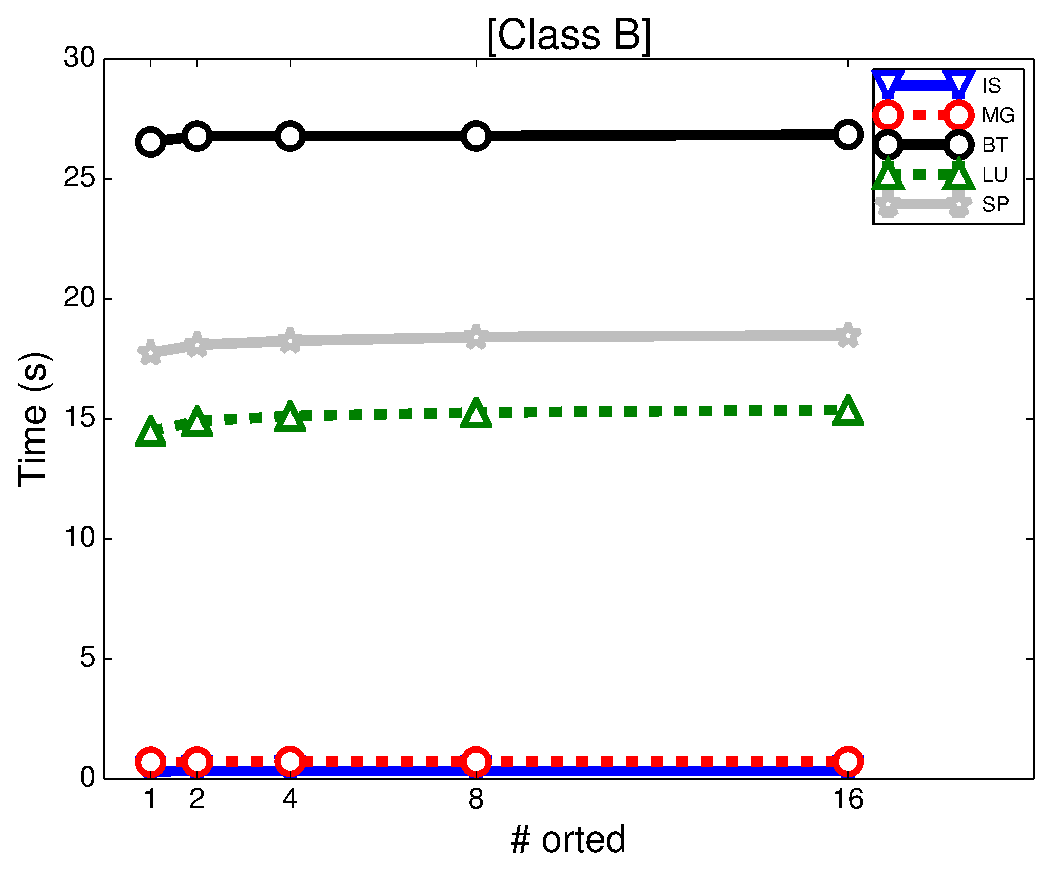
\includegraphics[scale=0.45]{img/orted_no_B_time.eps}
}
\hspace{3pt}
\subfloat{%
   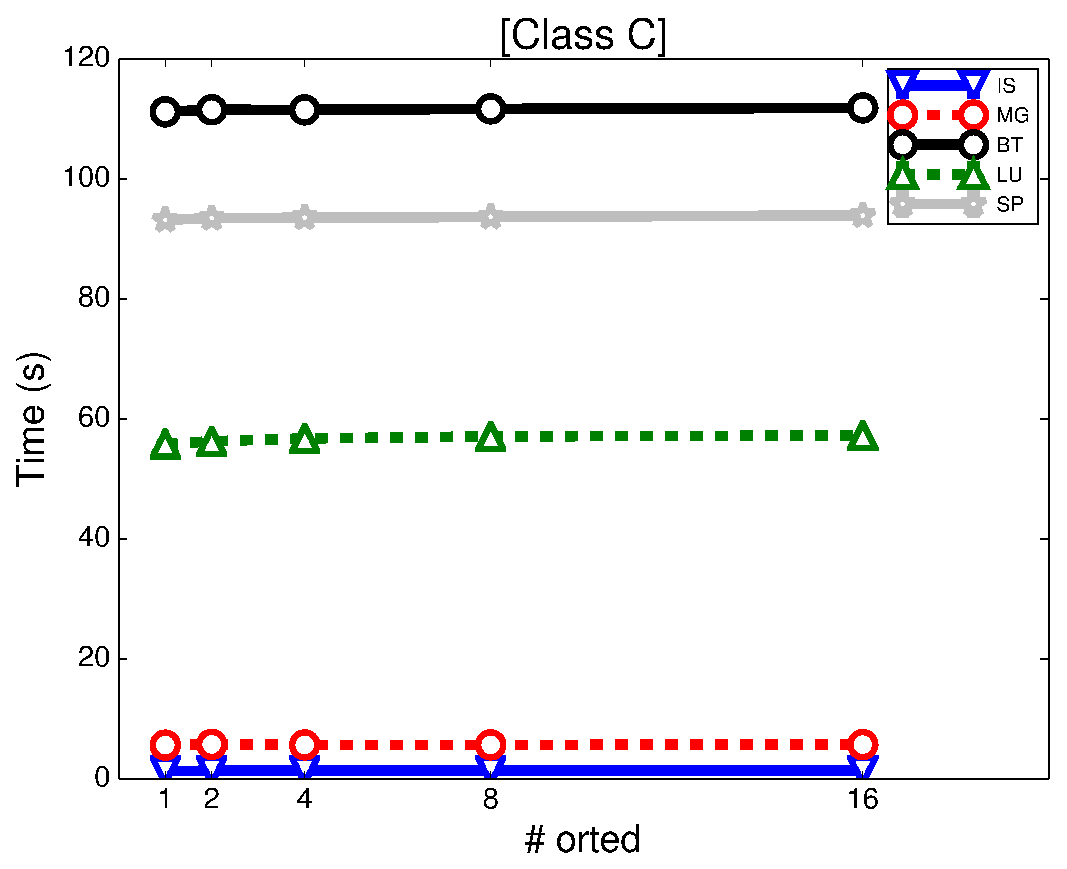
\includegraphics[scale=0.45]{img/orted_no_C_time.eps}
}
\hspace{3pt}
\subfloat{%
   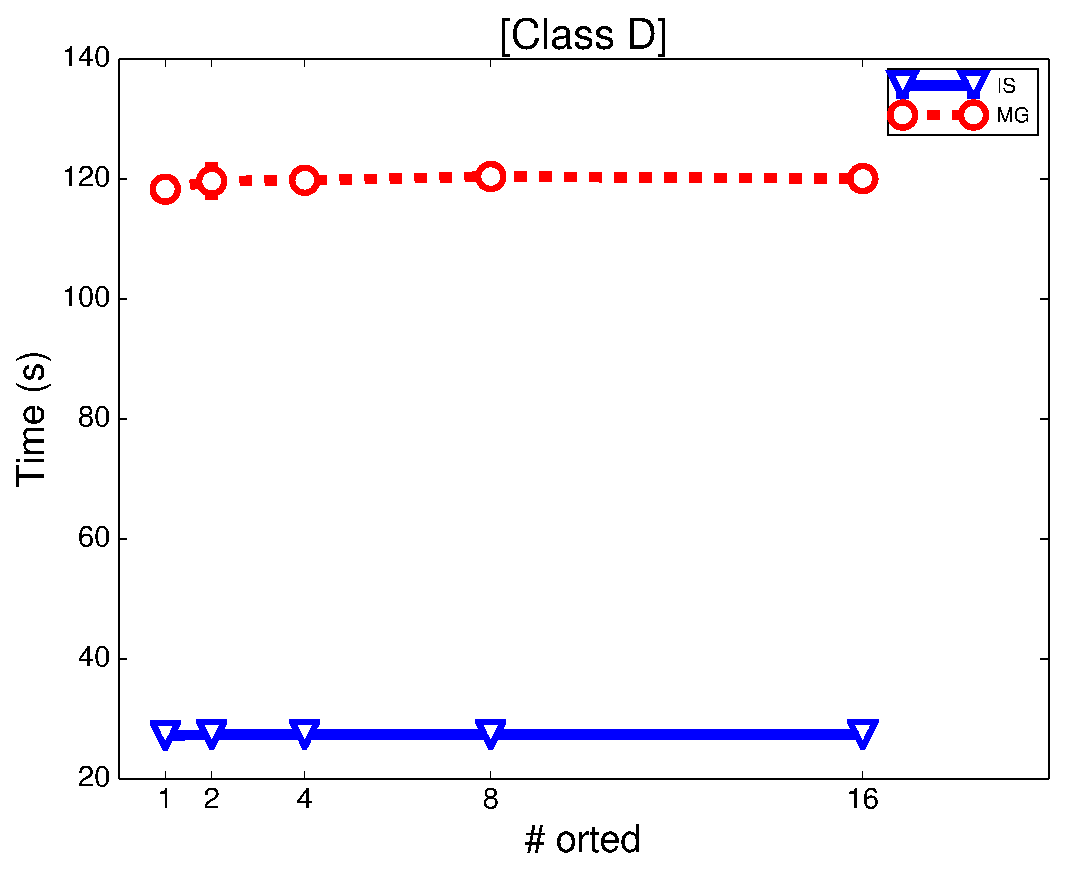
\includegraphics[scale=0.45]{img/orted_no_D_time.eps}
}
\caption[Multiple ORTE daemons benchmark]{Execution time of each benchmark when running 16 processes
using a number of \emph{ORTE daemons} that ranges from 1 to 16.}
  \label{fig:cap6-ortedstatic}%
\end{figure*}

\begin{table}[t]
\footnotesize
\centering
\begin{tabular}{c|c|c|C{2cm}} \hline
   \textbf{Benchmark} & \textbf{Class} &
   \begin{tabular}[x]{@{}c@{}}\textbf{\# orted}\end{tabular} &
         \begin{tabular}[x]{@{}c@{}}\textbf{Overhead} \textbf{\%}\end{tabular} \\ \hline

    \multirow{12}{*}{\texttt{IS}} & \multirow{4}{*}{B} & 2  & 4.68 \\
     &   & 4  & 5.18 \\
     &   & 8  & 4.85 \\
     &   & 16 & 4.85 \\ \cline{2-4}

     & \multirow{4}{*}{C} & 2  & 2.21 \\
     &   & 4  & 2.68 \\
     &   & 8  & 2.64 \\
     &   & 16 & 2.64 \\ \cline{2-4}

     & \multirow{4}{*}{D} & 2  & 0.87 \\
     &   & 4  & 0.96 \\
     &   & 8  & 0.79 \\
     &   & 16 & 0.64 \\ \hline

    \multirow{12}{*}{\texttt{MG}} & \multirow{4}{*}{B} & 2  & 1.28 \\
     &   & 4  & 4.36 \\
     &   & 8  & 1.73 \\
     &   & 16 & 3.24 \\ \cline{2-4}

     & \multirow{4}{*}{C} & 2  & 2.25 \\
     &   & 4  & 0.62 \\
     &   & 8  & 0.88 \\
     &   & 16 & 1.57 \\ \cline{2-4}

     & \multirow{4}{*}{D} & 2  & 1.13 \\
     &   & 4  & 1.25 \\
     &   & 8  & 1.79 \\
     &   & 16 & 1.50 \\ \hline

    \multirow{8}{*}{\texttt{BT}} & \multirow{4}{*}{B} & 2  & 0.92 \\
     &   & 4  & 0.93 \\
     &   & 8  & 0.93 \\
     &   & 16 & 1.17 \\ \cline{2-4}

     & \multirow{4}{*}{C} & 2  & 0.31 \\
     &   & 4  & 0.29 \\
     &   & 8  & 0.45 \\
     &   & 16 & 0.60 \\ \hline

    \multirow{8}{*}{\texttt{SP}} & \multirow{4}{*}{B} & 2  & 1.90 \\
     &   & 4  & 2.83 \\
     &   & 8  & 3.72 \\
     &   & 16 & 4.12 \\ \cline{2-4}

     & \multirow{4}{*}{C} & 2  & 0.31 \\
     &   & 4  & 0.40 \\
     &   & 8  & 0.52 \\
     &   & 16 & 0.79 \\ \hline

    \multirow{8}{*}{\texttt{LU}} & \multirow{4}{*}{B} & 2  & 2.92 \\
     &   & 4  & 4.37 \\
     &   & 8  & 5.42 \\
     &   & 16 & 6.10 \\ \cline{2-4}

     & \multirow{4}{*}{C} & 2  & 0.73 \\
     &   & 4  & 1.63 \\
     &   & 8  & 2.19 \\
     &   & 16 & 2.48 \\ \hline


\end{tabular}
\caption[Multiple ORTE daemons static overhead]{Static overhead of \texttt{IS}, \texttt{MG}, \texttt{BT}, \texttt{SP}, and \texttt{LU} with
increasing migration granularity, i.e. increasing number of \emph{ORTE daemons},
compared with single \emph{ORTE daemon} case.}
\label{tab:cap6-staticbench}
\end{table}

\clearpage


%% Migration composition
\begin{figure*}[t]
\centering
%\hspace{-53pt}
\subfloat{%
   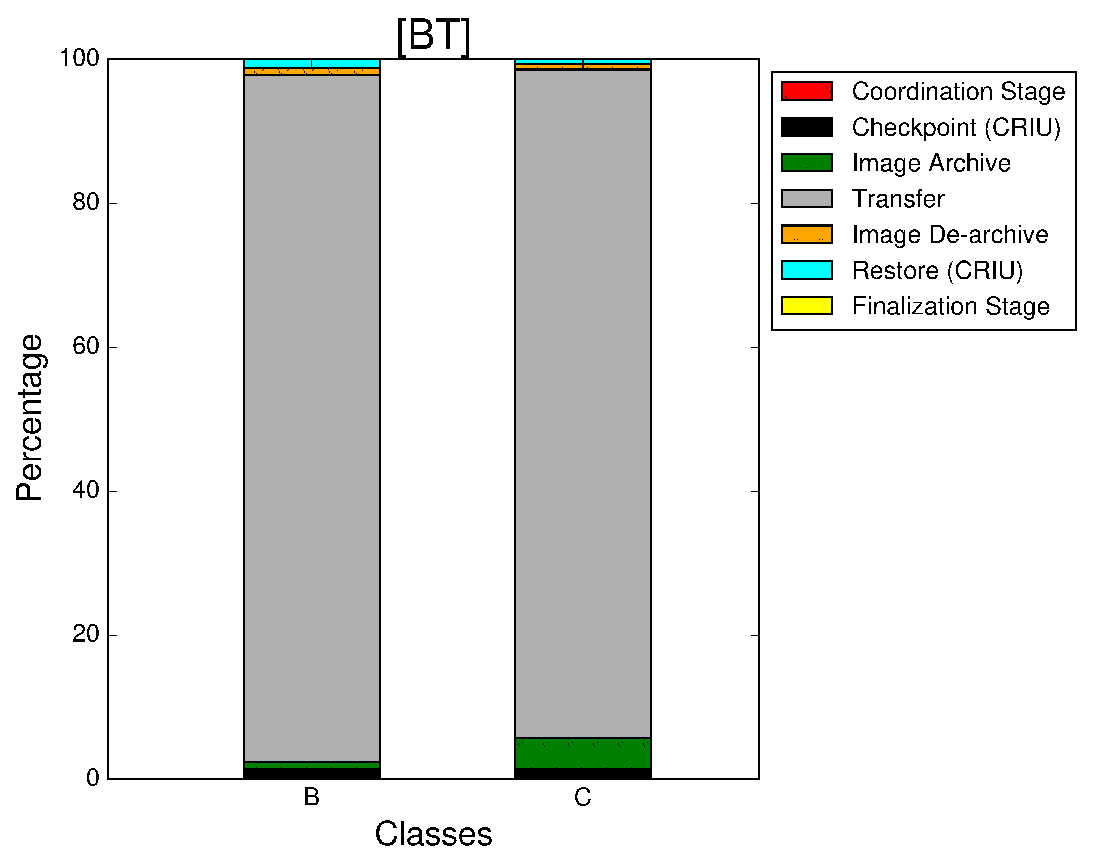
\includegraphics[scale=0.35]{img/migration_comp_bt.eps}
}
\subfloat{%
   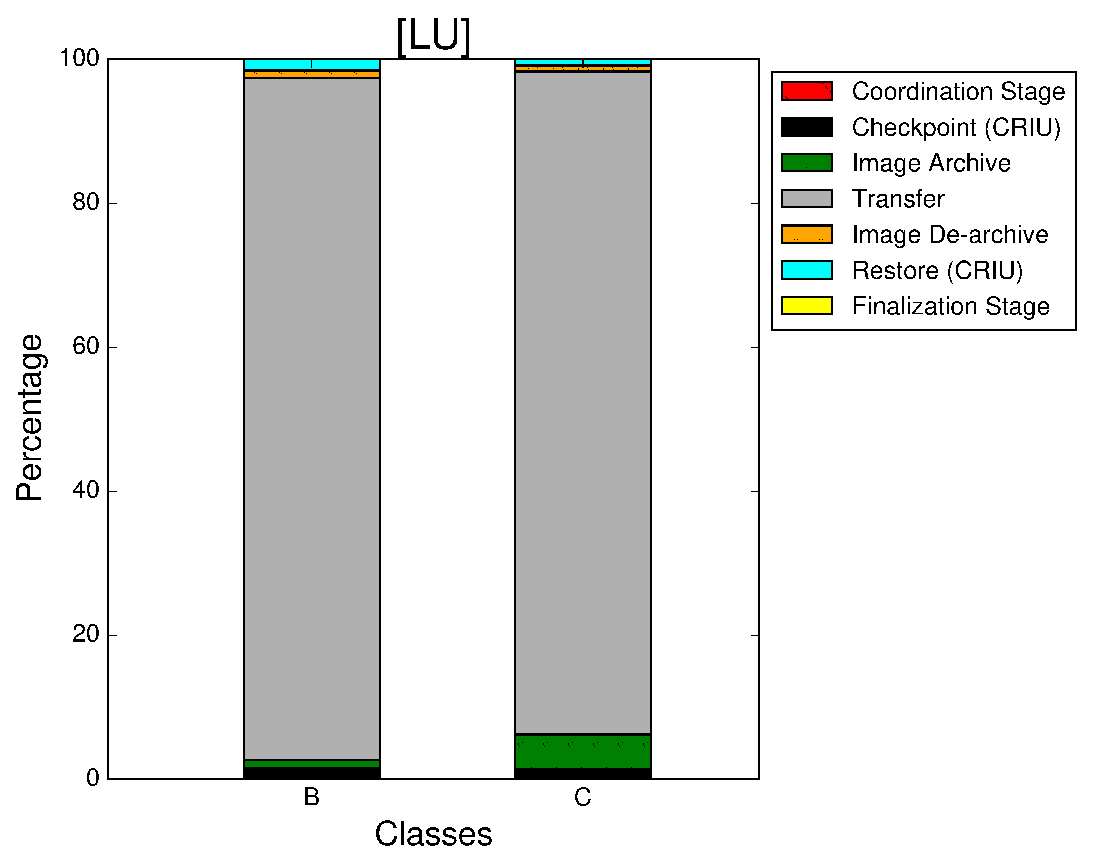
\includegraphics[scale=0.35]{img/migration_comp_lu.eps}
}


\vspace{10pt}

\subfloat{%
   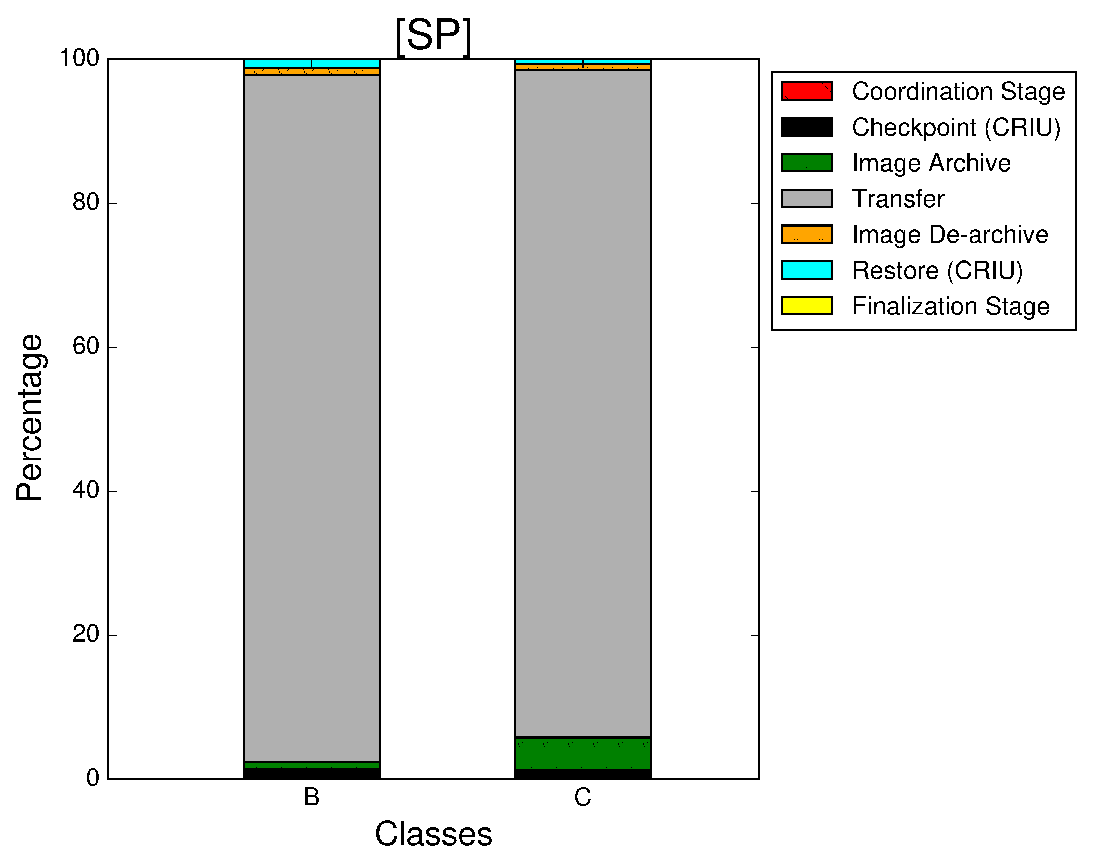
\includegraphics[scale=0.35]{img/migration_comp_sp.eps}
}
\subfloat{%
   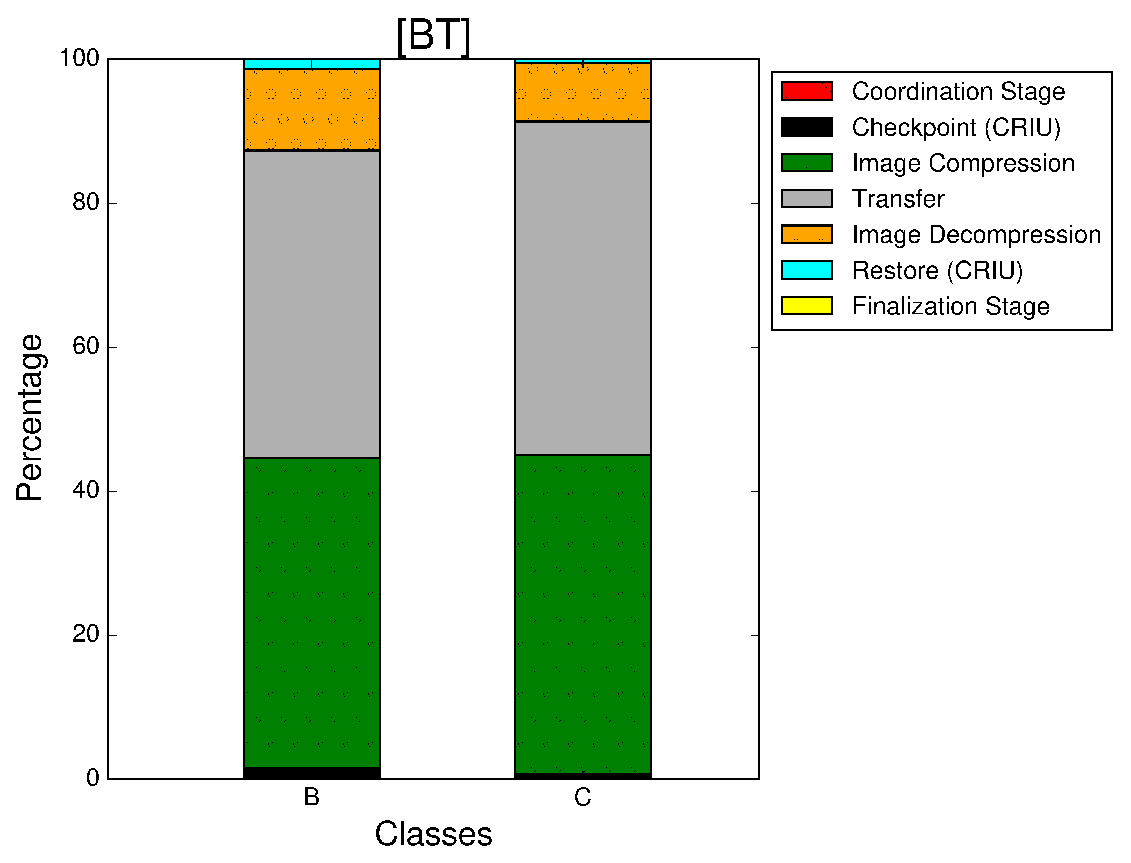
\includegraphics[scale=0.35]{img/migration_comp_bt_gzip.eps}
}

\vspace{10pt}

\subfloat{%
   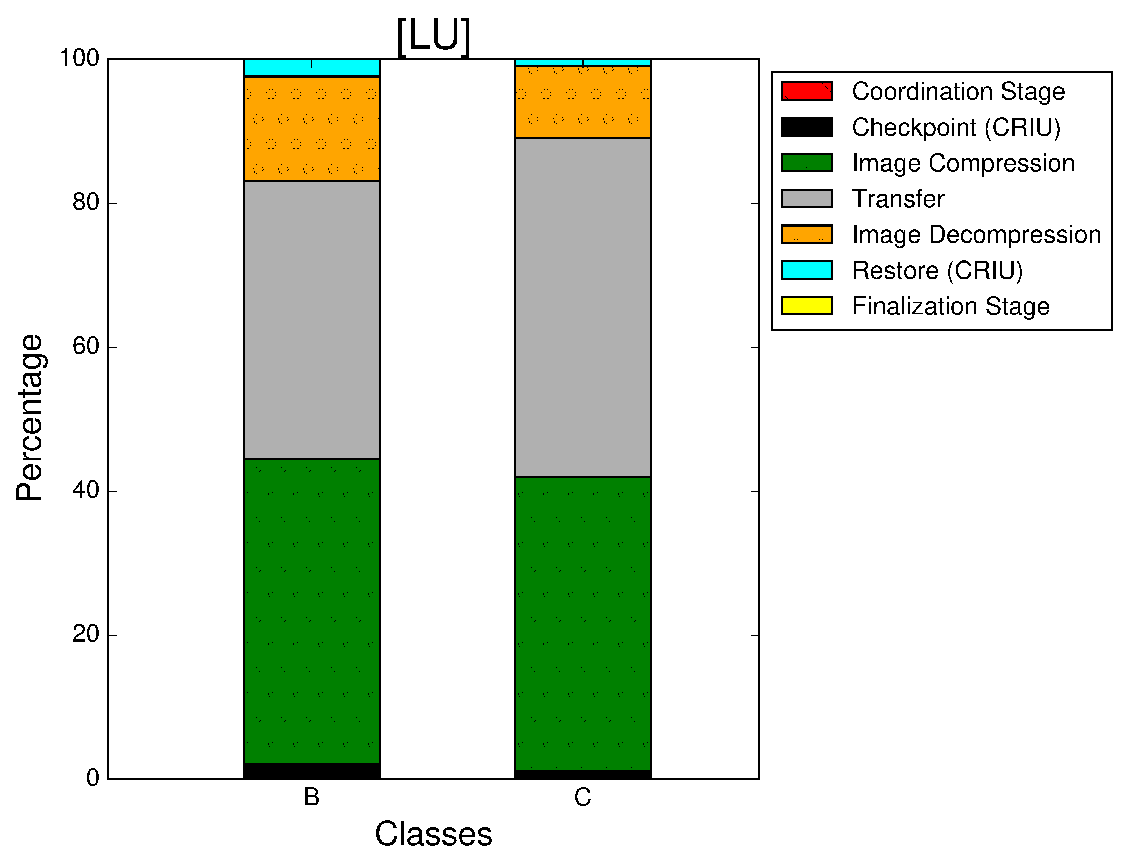
\includegraphics[scale=0.35]{img/migration_comp_lu_gzip.eps}
}
\subfloat{%
   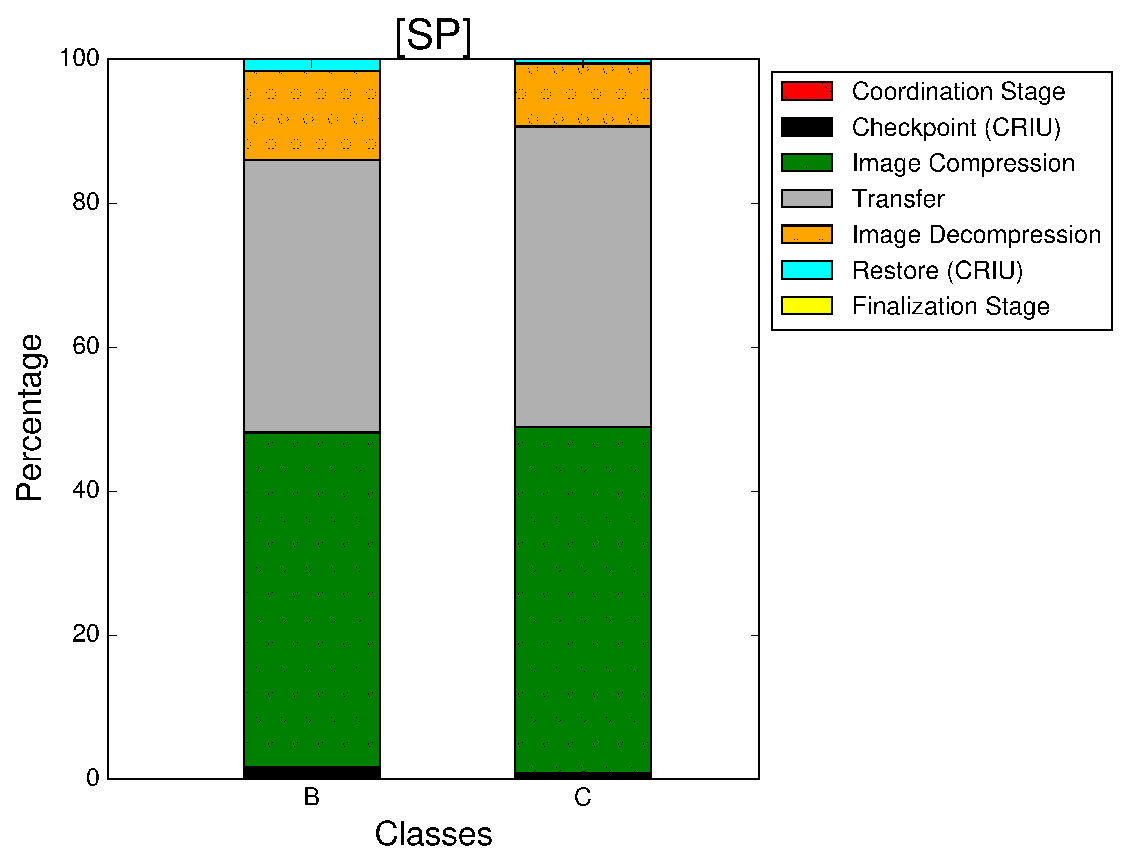
\includegraphics[scale=0.35]{img/migration_comp_sp_gzip.eps}
}
\caption[Process migration time composition]{Process migration time composition with respect to the input problem
size. Top images: migrations without image compression. Bottom figures:
migration  with image compression.}
  \label{fig:migrationstack}%
\end{figure*}

\clearpage

\section{\texttt{mig} : ORTE daemons migration overhead}
\label{sec:migoverhead}
\subsubsection{Hardware setup}
We characterized the migration overhead by
running the benchmarks on two nodes connected via Gigabit Ethernet, both
equipped with two Intel Xeon E5-2640 CPU, 128GB of RAM per CPU (NUMA) and
keeping the Hyper-Threading disabled.

\subsubsection{Methodology}

In the experimental migration scenario, we launched two \emph{ORTE daemon} instances
per node, each one managing 4 out of the 16 application processes. The
resource manager triggered the migration requests after 25 seconds of execution.

To better observe the composition of the migration overhead, we divided the
migration time, isolating seven contributions. We considered the time
required by each of the five migration phases previously described in \ref
{sec:cap4-migphases}, plus two additional contributions:
\begin{enumerate}
\item Time required to encapsulate the CRIU process dump into the archive;
\item Time to extract the dump from the archive after the migration.
\end{enumerate}

With the exception of the \emph{Coordination} and the \emph{Finalization}
phases, the other contributions are expected to be strongly dependent on the
problem size, in particular on the image transfer time.
In this regard, we evaluated the possibility of introducing the compression of
the image generated by the CRIU checkpoint before proceeding with the transfer.
In such a case, a decompression step is obviously required on the destination
node, before resuming the execution of the processes. To this purpose, we
used the GZIP compression algorithm \cite{deutsch1996gzip}.

\subsubsection{Results}

In Figure \ref {fig:cap6-imagesize}, we can see how the compression is effective in
reducing the size of the checkpoint image to transfer. This because of the
shared memory implementation. Open MPI in facts allocates over 100MB of unused
shared memory as ghost files initialized as zeros. The consequence is
that compression is very effective in such cases, resulting in image sizes
scaled down to $22-38\%$ with respect to the original sizes.
In case of bigger datasets instead -- like the \texttt{C} class -- this phenomenon
is less evident, with compressed image sizes resulting the $45-65\%$ of the
original sizes.

\begin{figure}[t]
\centering
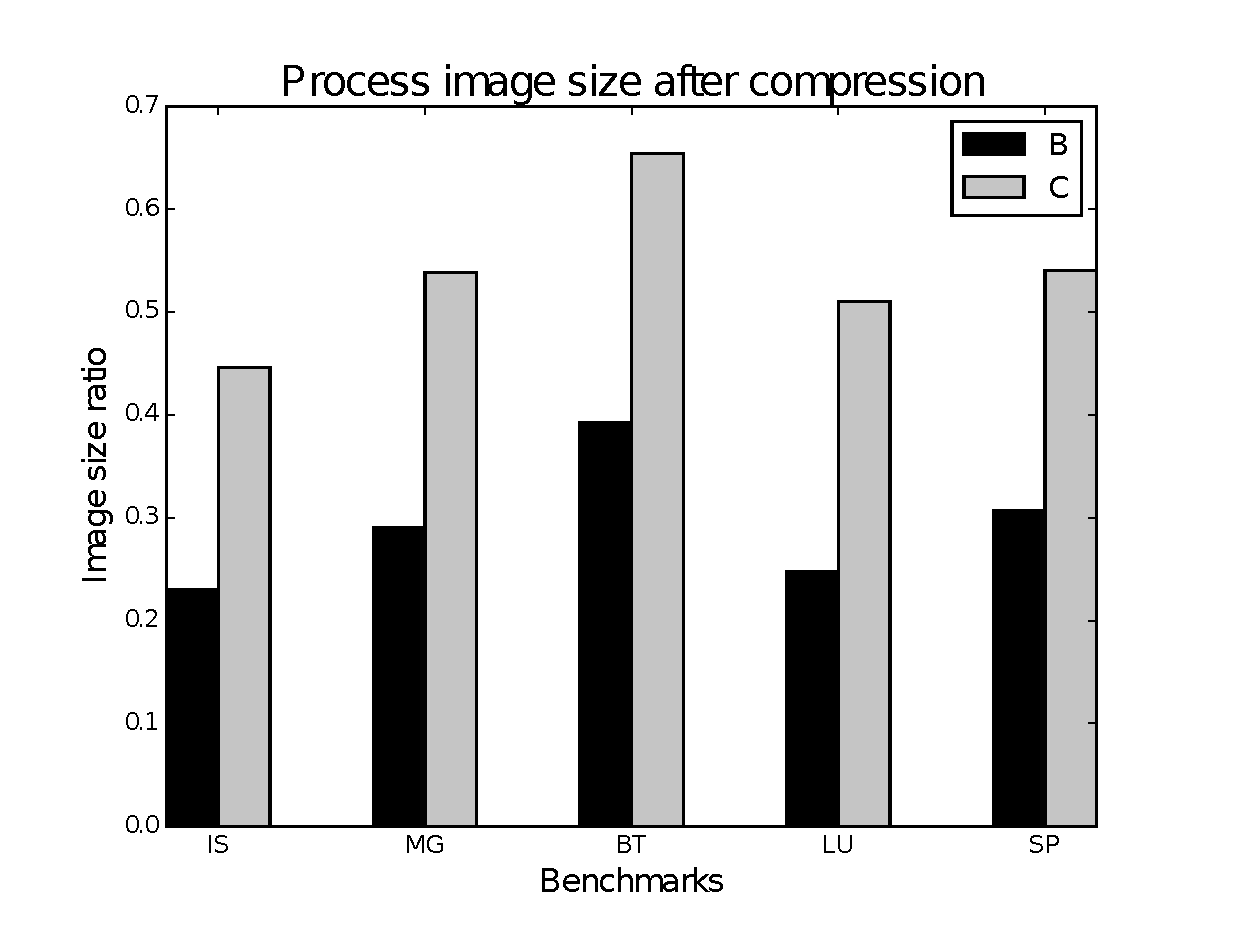
\includegraphics[scale=0.5]{img/image_size_per_data.eps}
\caption[Evaluation of the compression effectiveness]{Process checkpoint image after GZIP compression for each benchmark,
with respect to the input data class}
  \label{fig:cap6-imagesize}%
\end{figure}

The composition of the migration overhead is highlighted in Figure \ref
{fig:migrationstack}. If the compression is not applied (top figures), the time
required to transfer the process image over the network dominates the whole
migration process ($80-90\%$ of the time) independently of the benchmark and
of the class of input data. The contributions due to the synchronization stages
(\emph{Coordination} and \emph{Finalization}) and the time needed for doing
checkpoint/restore with CRIU are instead negligible.

Conversely, when the compression is applied (bottom figures), the transfer time
is reduced, but a new overhead contribution is introduced. The time spent to
perform image compression/decompression is not negligible. We can
observe indeed an overall percentage value comparable to the transfer time
($40-50\%$) for the compression, plus a $10-15\%$ for the decompression.

Figure \ref{fig:cap6-migrationtime} provides an overview of the
measured migration times, comparing the cases with image compression against
cases where no compression is applied. For the \texttt{IS} and \texttt{MG}
benchmarks, where hundreds of MB of data must be moved, the compression
represents a penalty. Conversely, for \texttt{BT}, \texttt{LU} and \texttt{SP},
where data size is a few MB, break-even points can be found.
Generally, we can state that resource manager should be in charge of choosing
whether apply compression or not, taking into account application properties, input
data size, node capabilities and network parameters (e.g., topology, bandwidth,
etc\dots). The \texttt{mig} framework is then driven accordingly.

\subsubsection{Comments}
Please note that these tests were performed on two computational nodes connected
via Gigabit Ethernet. Most recent HPC systems connect nodes using InfiniBand,
which is much faster than Ethernet. It follows that, in the average case, we do
not expect compression to be needed, because transfer time will usually be in
the range of seconds rather than of tens of seconds. In our experimental set-up,
as shown in the results, the time required to interrupt the execution of a set
of processes, to migrate them to another node and to resume their execution is
not negligible and may require tens of seconds.

%%% Migration time
\begin{figure*}[t]
\centering

\subfloat{%
   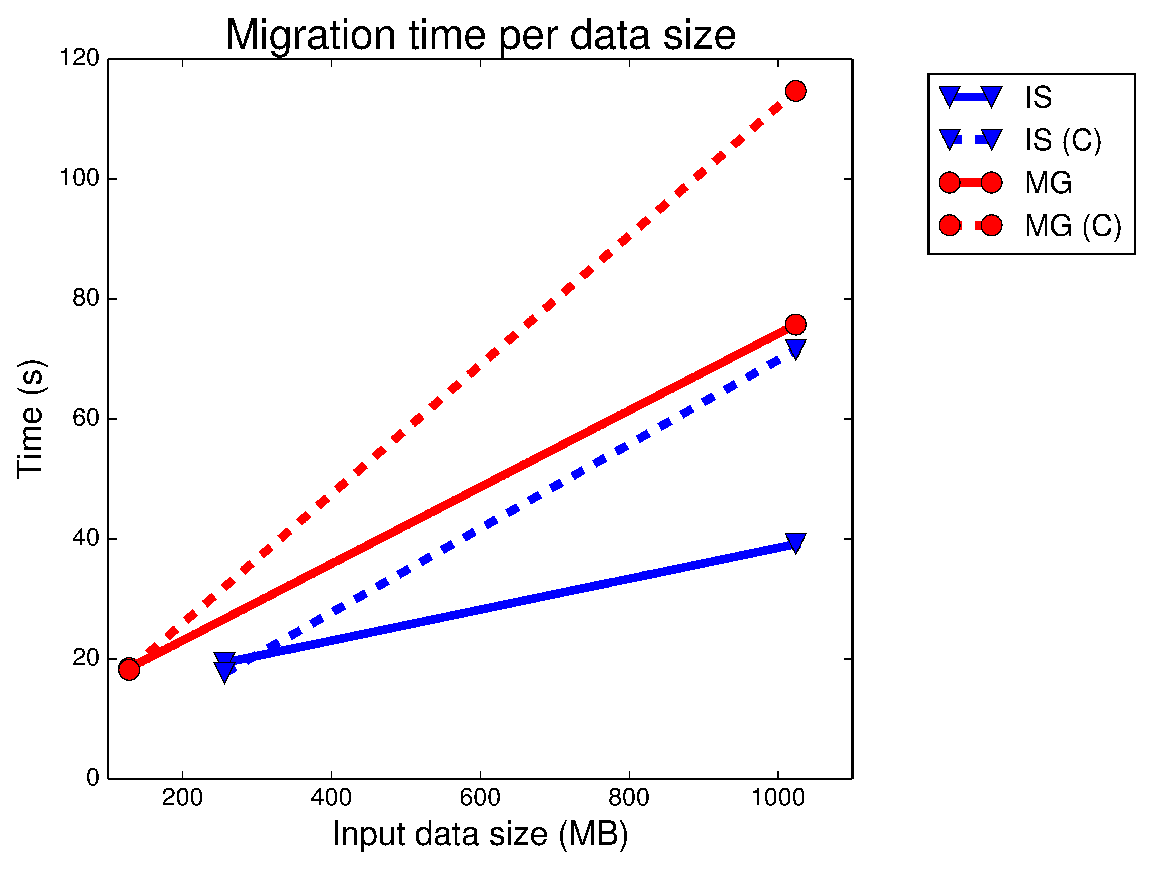
\includegraphics[scale=0.5]{img/migration_time_per_data_im.eps}
}
\hspace{10pt}
\subfloat{%
   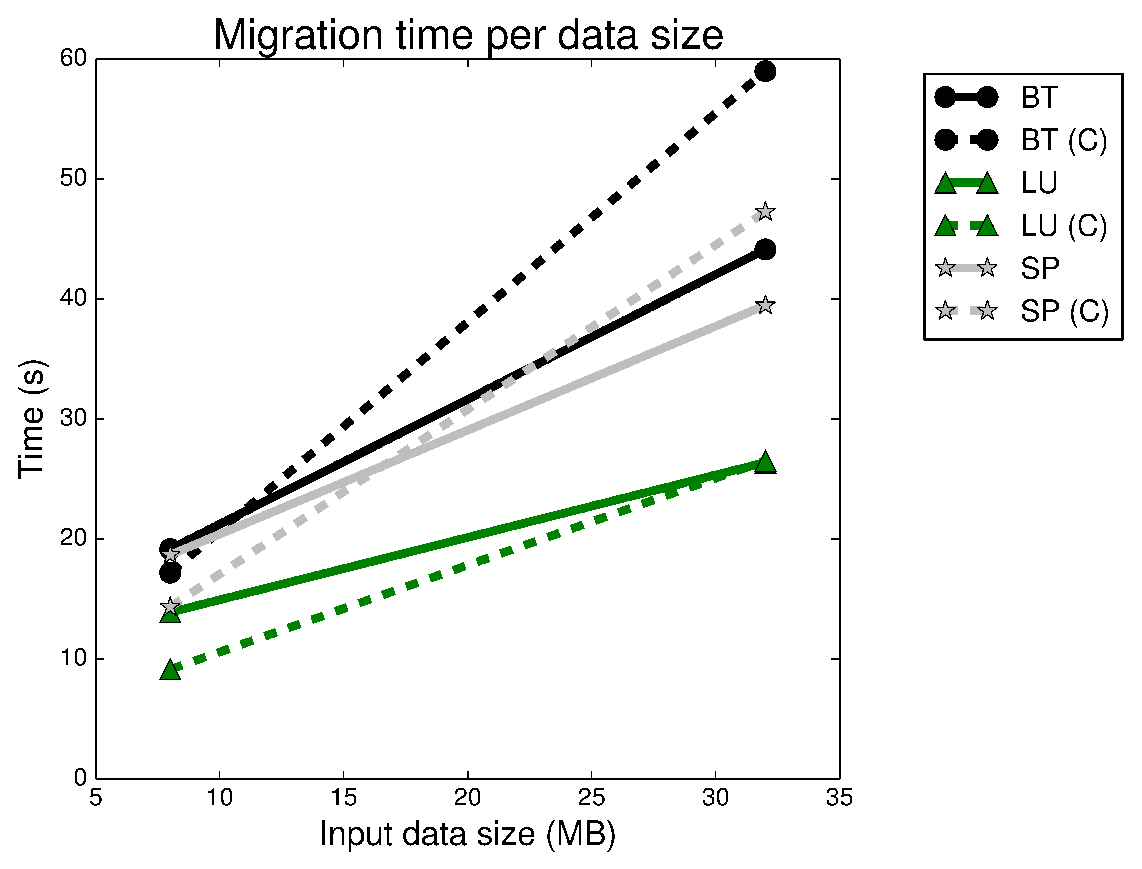
\includegraphics[scale=0.5]{img/migration_time_per_data_bls.eps}
}
\caption[Migration overhead evaluation]{\texttt{IS}, \texttt{MG} and \texttt{BT}, \texttt{SP}, \texttt{LU}
    migration overhead with respect to the input problem size. Migrations using image
    compression (dashed lines (C)) can be compared to migrations without image
    compression.}
  \label{fig:cap6-migrationtime}%
\end{figure*}

\clearpage

\section{DistRib validation}
\label{sec:distribval}

\begin{figure}[t]
    \centerline 
{\includegraphics[scale=0.4]{img/ilp-1-cropped.pdf}}
    \caption[DistRib ILP performance (no per-system penalty)]{Performance results of ILP problem with homogeneous systems (no
    per-system penalty).}
    \label{fig:cap5-ilp_nopen}
\end{figure}


\begin{figure}[t]
    \centerline 
{\includegraphics[scale=0.4]{img/ilp-2-cropped.pdf}}
    \caption[DistRib ILP performance (per-system penalty)]{Performance results of ILP problem with heterogeneous systems 
    (per-system penalty presents).}
    \label{fig:cap5-ilp_pen}
\end{figure}

\subsection{The GLPK solver}
In order to solve the ILP problem the
\textbf{GNU Linear Programming Kit (GLPK)}
\cite{makhorin2008glpk} is used. GLPK implements Linear Programming (LP) and
Mixed Integer Programming (MIP) solvers. The latter is a generalized case of 
ILP, since it allows the mix between integer and real variables. Since the
textual formulation presented in Appendix \ref{app:distrib-ilp-formulation}
is adequate
only for the first prototype of the ILP formulation, the actual code uses the 
API provided by GLPK itself, linking the relative shared library.

\subsubsection{The algorithms used}
GLPK implements several algorithms for the resolution. The policy uses the
standard \emph{Simplex algorithm} for solving the LP relaxation and then the
\emph{branch-and-cut} method \cite{mitchell2011branch} to obtain the integer
solutions. The \emph{branch-and-cut} method is a hybrid of classical
\emph{branch-and-bound} and \emph{cutting plane} methods that assure an
optimal solution with a good probability. GLPK allows the production of a 
sensitivity report in order to analyze the goodness of the solution, however
at present this is not used in our software.

\subsection{Performance}

Integer Linear Programming is proved to be \emph{NP-complete}
\cite{papadimitriou1981complexity}, thus no\linebreak polynomial-time
algorithm is known.

We performed the tests timing GLPK solver.
The instances are selected from 1 to 20 systems and from 1 to 20 applications,
for a total of 400 instances. The number of cores per system and the number
of cores per application are uniformly randomized. Each instances are executed
20 times and the resulting execution times have been averaged. A timeout at
20 seconds is placed, after that the execution is killed.

The first batch of tests are executed with \(r_s=0\ \forall s \in S\)
(homogeneous systems) and the results presented in Figure
\ref{fig:cap5-ilp_nopen}. The second batch
of tests are executed with \( r_s \) as a random value from 1 to 10
uniformly distributed. This test implements the case of heterogeneous systems and its results presented in Figure 
\ref{fig:cap5-ilp_pen}.
The two cases do not show any significant difference adding the addend of
per-system penalty to the objective function.

However, GLPK performs well with our ILP programming for number of applications
less than 10, and it seems not very sensitive to the number of systems.
Isolated cases are very fast even with a high number of systems and
applications. For example, \emph{(15 applications, 17 systems)} is very fast
case, but \emph{(14 applications, 17 systems)} and \emph{(16 applications,
17 systems)} are very slow. This behavior may be explained analyzing the
optimization performed by GLPK, that can solve rapidly some special cases.

In a real HPC scenario with thousands of nodes and several applications
a greedy policy or other non optimal algorithm is required. The policy has to
be sufficiently fast in order to do not introduce more overhead.


\chapter{Future Works and Conclusions}
\label{cap:discussion}
This final chapter summarized the goals that have been achieved with this project and provides an overview of the possible future works regarding the tool, how can it be expanded and what can be improved.

The world of \emph{self adapting systems} has been studied only in the last few years in order to answer the request of the users that demanded software which can adapt to their needs. For this reason there are no universally recognized metrics that can be used to evaluate such systems.

This project was born with the goal to provide some metrics and a tool that help in deciding which component to purchase or develop when designing an architecture, understand which are the disadvantages in favoring one quality attribute over another and limit the drawbacks that this behavior produces.

The biggest limit of all the previous studies is that they analyze the architecture only from a static point of view; this tool has further strengthened this studies and has expanded them by adding the analysis of the architecture with some metrics that can also study the dynamic behavior of the system by using a sequence diagram. 

For some metrics the need to optimize the algorithms was born in order to reduce computation times, especially when architectures have many components; this was done by an exhaustive study of the problem and modeling  the algorithms in such a way that they can provide in the average case results in a reasonable time without sacrificing completeness.

It was also developed in a modularized way that makes further developing easy and reduce the burden of future refactoring.

\section{Future Works}
The last implementation of the tool, despite being fully functional in its features, has some features that a final analysis found can be improved or changed but they were left as they are for a lack of time even if the code have been written in a way that should make these changes easy to implement.

\subsection{Services in a Component}
Some metrics, for sake of simplicity in writing the formulas, don't take in consideration that one component can provide more than a service. The Java object for the component already take into account multiple Provided Services but some metrics just ignore that.

\subsection{Paths}
In the actual implementation of the sequence diagram is not possible to nest multiple paths in order to represent nested \texttt{Alt} and/or \texttt{Opt} blocks. To implement this feature the structure of the Java code of the \texttt{Workflow} and \texttt{Path} should be revised.

Also the tool does not check the correctness of a path when a message is entered, such as if a message \texttt{S1 -> S2} exists but no component that provides S1 also requires S2 exists in the architecture.

\subsection{Adaptability}
Some more tabs can be added in the tool to expand the analysis of the adaptability with respect to other quality metrics other than cost. This can be achieved by implementing some other metrics and calculations in order to display the appropriate graphs.

\subsection{Visual representation of the architecture}
When displaying the graphical representation of the architecture, all the components are positioned at random in the window. The actual code provides a way to implement a new Java class that can place the components with an order.


\begin{appendices}

\end{appendices}


\cleardoublepage
\phantomsection
\addcontentsline{toc}{chapter}{\bibname}
\small
\bibliographystyle{unsrt}
\bibliography{thesis}



\end{document}
